\documentclass[article]{jss}

\author{
Grant Cavanaugh, Ph.D.\\Praedicat \And Benjamin Collier, Ph.D\\Wharton
}
\title{Developing Direct Climate Markets: Pricing Uncertainty in ENSO Forecasts}
\Keywords{climate, risk, finance, insurance, ENSO}

\Abstract{
Existing markets struggle to provide direct, reliable protection against
longer-dated climate risks. This paper discusses how financial markets
for indexes of regional climate anomalies with long-range physical and
statistical links to extreme weather events, or what climate scientists
call \emph{teleconnections}, can address that market gap. Quantifying
teleconnection risk requires estimating errors in regional climate
forecasts. To that end, we provide a framework and tools to incubate
risk trading for the best known teleconnection index, El
\text{Ni\~no}-Southern Oscillation (ENSO). We suggest that the social
gains from markets in teleconnection risk in general, and ENSO in
particular, are high if such markets feature active trading because such
trading can effectively respond to emerging information and generate
actionable forecasts of climate risk.
}

\Plainauthor{Grant Cavanaugh, Ph.D., Benjamin Collier, Ph.D}
\Plaintitle{Developing Direct Climate Markets: Pricing Uncertainty in ENSO Forecasts}
\Shorttitle{Direct Climate Markets}
\Plainkeywords{climate, risk, finance, insurance, ENSO}

%% publication information
%% \Volume{50}
%% \Issue{9}
%% \Month{June}
%% \Year{2012}
%% \Submitdate{2012-06-04}
%% \Acceptdate{2012-06-04}

\Address{
    Grant Cavanaugh, Ph.D.\\
  Praedicat\\
  5760 W. Jefferson Los Angeles, California 90016\\
  E-mail: \href{mailto:grant.cavanaugh@praedicat.com}{\nolinkurl{grant.cavanaugh@praedicat.com}}\\
  URL: directclimatemarkets.com
    }

\usepackage{amsmath} \usepackage{graphicx}

\begin{document}

\section{Introduction}\label{introduction}

Financial risk management tools that manage the risk of global climate
change could reduce suffering and loss, both directly, via hedging, and
indirectly, by generating valuable information that can support policy
(B. Collier and Skees 2013). However, few if any such tools are
available. While there are many markets today where firms and
individuals can trade or manage risk influenced by climate, it is
difficult to identify existing markets that offer direct, reliable
protection against longer-dated climate risks.

Among the better known traded markets with some link to climate are
those for emission permits, temperature and rainfall derivatives
covering major cities, and equities for companies in weather dependent
industries. Similarly, there are markets for insurance and reinsurance
risks, influenced by climate, that are traded by specialized
institutional investors (Kurtov 2010). But none of these markets offer
at-risk communities direct protection from climate extremes at
competitive prices representing an informed forecast of global weather
patterns.

Prices on these markets are primarily driven by non-climate factors,
such as policy or recent returns in bond and equity markets (The
Economist 2013; Kurtov 2010). This means that companies or individuals
looking to hedge actual climate risk on existing markets may find that
their best available proxies for climate risk bear little resemblance to
their actual experience of that risk. In the language of finance, these
\emph{cross hedges} show \emph{high basis risk}.

Even when price in these existing markets explicitly reflect long-term
climate considerations, they often fail to do so directly. This means
that it is difficult to use the resulting prices to forecast climate
events. Take for example, an index-based insurance settling exclusively
on rainfall measured at specific weather station. Such a risk product
removes practically all factors except the weather risk and its drivers,
such as changing climate. So, a reinsurance company offering this
protection must explicitly account for climate in their price. But, even
in pricing such a simple product, a reinsurer will often use an
\emph{uncertainty load}, a heuristic to adjust their best price estimate
upward to reflect uncertainty, rather than make an explicit and
rigorously researched forecast of the link between climate and a
localized index.

Markets could expand to cover the indexes most assocaited with long-term
global climate change, like the extent of Arctic ice or global mean
surface temperatures. But many of these indexes are ill-suited to formal
risk management. First, meaningful changes in these indexes unfold over
a long time horizon relative to the planning horizons of commercial and
public decision makers ({IPCC} 2013). That mismatch complicates
climate-related collective action in general and would likely check the
provision of liquidity on a traded market. Moreover, it may also pose a
challenge to individual economic experts evaluating the merits of
hedging climate risk (Jacquet et al. 2013; Nordhaus 2013; Pindyck 2013).

But even if the horizons of trends in these primary climate indicators
matched the horizons over which organizations made formal risk
management decisions, these indexes would be difficult to translate into
forecasts of adverse climate events on a geographic scale that is
actionable for individual firms and organizations. Firms tend to hedge
risks through using formal financial tools only when their risk managers
understand how adverse changes in the index underlying a hedge will
imperil specific contractual relationships (Pennings and Leuthold 2000;
Pennings and Leuthold 2001). Global climate models, such as those that
support much of the analysis in the UN's IPCC reports, often do not
include analysis with that level of geographic specificity. While there
have been advances in \emph{downscaling}, translating long-term climate
models into regional forecasts, it is difficult to access their validity
because of the long time horizon of the changes predicted (Fowler,
Blenkinsop, and Tebaldi 2007). These models differ starkly from the
types of models used commonly used to reinsure property against
catastrophic natural disasters like hurricanes or earthquakes, which can
be tested and improved on an ongoing basis.

Finally, while the link between global climate indexes and regional
weather remains uncertain, many of the tends in those global indexes are
considered highly likely. For example, the ({IPCC} 2013) notes with
virtual certainty (a \textgreater{}99\% chance) that sea level rise will
continue beyond 2100. Such certainty also undermines some climate
indexes' value for formal risk management. Financial risk transfer is
generally not suitable for managing known outcomes but instead focuses
on managing the risk around uncertain outcomes. As the saying goes,
insurance is very expensive once the house is on fire. Known, or highly
certain outcomes, such as sea level rise, are traditionally managed
through risk mitigation (building levees, relocating populations, etc.)
rather than risk transfer.

Together, the difficulties of building meaningful financial contracts
directly around climate change and the basis risk inherent to managing
climate risk with existing markets suggest a missing market for
financial contracts that could:

\begin{itemize}
\itemsep1pt\parskip0pt\parsep0pt
\item
  Directly cover climate risks rather than simple short-term weather
  indicators;
\item
  Meet conditions associated with stable financial risk transfer flows,
  such as a minimum level of volatility in the underlying index (Working
  1953; Silber 1981; Carlton 1984; D. Black 1986; Duffie and Jackson
  1989; Tashjian 1995; Pennings and Leuthold 1999; Brorsen and Fofana
  2001; Gorham and Kundu 2012; Sandor 2012); and
\item
  Fit within the actionable geographic scope and time horizons of
  decision makers attempting to prepare for a changing climate.
\end{itemize}

This paper discusses how financial markets for indexes of regional
climate anomalies with long-range physical and statistical links to
extreme weather events, or what climate scientists call
\emph{teleconnections}, fit well into that market gap.

Teleconnection risk indexes including El \text{Ni\~no}-Southern
Oscillation (ENSO) and the Artic Oscillation do not suffer from the
basis risk inherent to many longer range climate indicators. They can be
directly and sometimes causally linked to extreme weather in specific
communities. Hence these climate drivers are specific enough to worry
individuals, firms, and institutions in the short-term. Yet, they are
also long-dated and wide-ranging phenomenon, so they have a clearer
connection to global climate change than localized weather indexes.

The analysis presented here is focused on the prospects for ENSO markets
in particular, however it also addresses questions broadly applicable to
risk markets sitting at the intersection of finance and science, such
as:

\begin{itemize}
\itemsep1pt\parskip0pt\parsep0pt
\item
  When is a scientific risk well suited to direct management on a traded
  market?
\item
  How can a new science-driven risk market avoid the asymmetric
  information problems that could undermine active trading?
\item
  When do scientific forecasts contain financially actionable
  information?
\item
  How can we incorporate multiple sources of scientific uncertainty into
  risk markets?
\item
  Does a given risk have informative emerging forecasts and sufficient
  underlying volatility to drive active trading?
\end{itemize}

ENSO (more specifically the Oscillation's extreme anomaly events called
El \text{Ni\~no}/La \text{Ni\~na}) is a climate driver with
teleconnections whose risk is already directly managed through an
innovative insurance (Skees 2013). With support from the Gate
Foundation, the authors were involved in the design, pricing, and sales
of that insurance. The El \text{Ni\~no} insurance market is noteworthy
in that it is the first market to directly hedge teleconnection risk and
has been structured as forecast insurance - an insurance that pays based
on a remotely measured geophysical event that precedes much of El
\text{Ni\~no}'s physical damage.

This new ENSO insurance provides the direct protection against regional
climate anomalies. However, ENSO and other similar regional climate
phenomenon with teleconnections, share some characteristics that may
ultimately leave their risk more efficiently managed via traded markets.
This article discusses the benefits of managing teleconnection risk on
traded markets. It also discusses how ENSO risk, should it succeed in
moving to a traded market, would set a precedent for a suite of markets
providing a robust foundation for climate risk adaptation and mitigation
strategies. Those markets would generate prices containing socially
valuable forecast information.

We also introduce a pricing framework that is necessary but not
sufficient to catalyze early trades those markets. This framework will
give benchmark prices to risk managers seeking climate protection, even
as new forecast information becomes available. Dealing with such
forecast information and placing a price on the uncertainty within
available forecasts is a critical hurdle for the development of robust
direct climate markets. Indeed the information asymmetries associated
with ENSO forecasts have complicated the sale of existing insurance
against extreme El \text{Ni\~no} in Peru, which we helped design and
sell with support from the Gates Foundation.

\section{Identifying appropriate instruments to manage climate
risks}\label{identifying-appropriate-instruments-to-manage-climate-risks}

El \text{Ni\~no}/La \text{Ni\~na} is characterized by a host of physcial
characteristics that have profound implications for how the phenomena's
risk can be efficiently managed:

\begin{itemize}
\itemsep1pt\parskip0pt\parsep0pt
\item
  Simple index - ENSO anomalies are measured by a relatively simple
  index.
\item
  Index anomalies linked to distinct risk events - Anomalies in SSTs
  translate to discrete risk outcomes that are well understood by
  at-risk communities.
\item
  Spatially correlated risk - ENSO risk is spatially correlated.
\item
  Cyclical risk - ENSO has an annual cycle.
\item
  Forecasts have social value - Individuals and policy makers use
  forecasts of ENSO SST to prepare for disasters.
\item
  Offsetting pools of risk - ENSO is associated with potentially
  offsetting consequences across regions and time.
\item
  Few opportunities for arbitrage - There are few simple, reliable
  proxies for ENSO risk that are/could be traded.
\end{itemize}

These characterisics (particularly the simple index, links to distinct
risk events, and spatially correlated risk) allowed GlobalAgRisk to
create an innovative El \text{Ni\~no} insurance (Khalil et al. 2007).
However, these characteristics, many of which ENSO shares with other
teleconnection-linked anomalies, also suggest why ENSO risk may
ultimatly be more efficiently managed through traded markets.

After a brief introduction to ENSO, we discuss each of these
characteristics individually and how they favor some risk management
solutions, such as exchange-traded derivatives or catastrophe bonds,
over others. Given the qualitative similarity between ENSO and other
teleconnection indexes, the following section provides a general
framework for choosing the appropriate financial instruments for any
direct climate market.

\subsection{Introduction to ENSO risk}\label{introduction-to-enso-risk}

ENSO refers to a coupled oceanic/atmospheric cycle. In normal years, the
cycle follows currents and winds (each reinforcing the other) as they
bring water along the surface of the Pacific Ocean from South America
(the eastern side of the Pacific) to Indonesian and the South Pacific
(the western side of the Pacific). As that water travels along the ocean
surface, it warms. The resulting mass of warm water sinks as it arrives
in the western Pacific and begins circulating back toward Peru along the
cold ocean floor. The cycle ends with cold water rising to the surface
in the eastern Pacific, sustaining rich fishing grounds off the coast of
Peru and Chile (Clarke 2008).

During an El \text{Ni\~no} anomaly, this cycle weakens. Usually starting
in March or April, a plume of warmer-than-normal water creeps eastward
across the Pacific, lessening the normal temperature gradient from the
Western to the Eastern Pacific. When that plume of warmer-than-normal
water reaches Peru, usually by January, it parks a moisture laden air
mass off the South American coast. When that mass air meets the cold air
descending from the Andes, it causes an extended period of torrential
rains and flooding in northern Peru and southern Ecuador (Lagos et al.
2008).

By contrast, during a La \text{Ni\~na} anomaly the normal cycle
enhances. More water gets pushed from the South American coast, raising
sea-surface temperatures in Australia and Indonesia above normal. That
leaves Southeast Asia and Oceania with increased incidence of extreme
rains and flooding (Chiew et al. 1998).

\subsection{Simple index}\label{simple-index}

National Meteorological Services (NMS) monitor El \text{Ni\~no}/La
\text{Ni\~na} by measuring sea-surface temperatures (SST) over defined
regions of the Pacific Ocean. That means that the the phenomenon can be
accurately expressed using freely available data, provided in
simple-to-understand units (degrees centigrade), according to a
methodology that is well defined (Khalil et al. 2007). These qualities
are attractive to prospective market speculators (those that might offer
El \text{Ni\~no} protection in exchange for an expected profit), because
they mitigate many of the moral hazard and adverse selection problems
inherent to traditional insurance (Skees, Black, and Barnett 1997).

Catastrophic risk professionals would welcome the opportunity to price
protection using the simple, reliable, and inexpensive data that
describe ENSO and many other teleconnection indexes. Both the realized
and opportunity costs of writing that protection are low compared to
most catastrophic risks, which tend to be inherently multi-variate (Woo
1999). Hurricane risk for example, even represented as a standardized
index, requires estimates of windspeeds, storm track, and the time that
a storm will spend over a given area (CME Group 2014). This is
sufficiently complicated that even sophisticated hedge funds
specializing in catastrophic risk rely on third-party catastrophe models
from specialist firms like RMS, AIR Worldwide, and EQECAT.

The simplicity of ENSO SST indexes facilitated the launch of
GlobalAgRisk's initial insurance, allowing reinsurers to confidently
price protection using only the expertise of their existing modelers. If
indeed the risk eventually moves to traded markets, the same simplicity
will allow new speculators interested in selling protection for an
expected profit to enter the market quickly.

\subsection{Index anomalies linked to distinct risk
events}\label{index-anomalies-linked-to-distinct-risk-events}

While speculators' prefer to sell protection on simple and reliable
indexes, those characteristics are not enough to drive hedgers (those
looking to transfer risk for expected loss) to use a new risk market. To
entice hedgers a risk market's underlying index must correspond tightly
to hedgers' risk perceptions (Ederington 1979). That is indeed the case
for NOAA's SST indexes. Anomalies in SSTs translate to discrete risk
outcomes that are well understood by at-risk communities.

Perceived basis risk is particularly low for Peruvian hedgers managing
the risk of catastrophic flooding in the country's Northern region using
SST measurements from the \text{Ni\~no} 1.2 region, directly off the
Peruvian coast as shown in figure \ref{fig:ninoareas}. In fact, the high
SSTs measured by NOAA's various indexes are the immediate physical cause
of flooding, so the link between the index and risk outcomes is more a
simple statistical association (Khalil et al. 2007).

\begin{figure}
  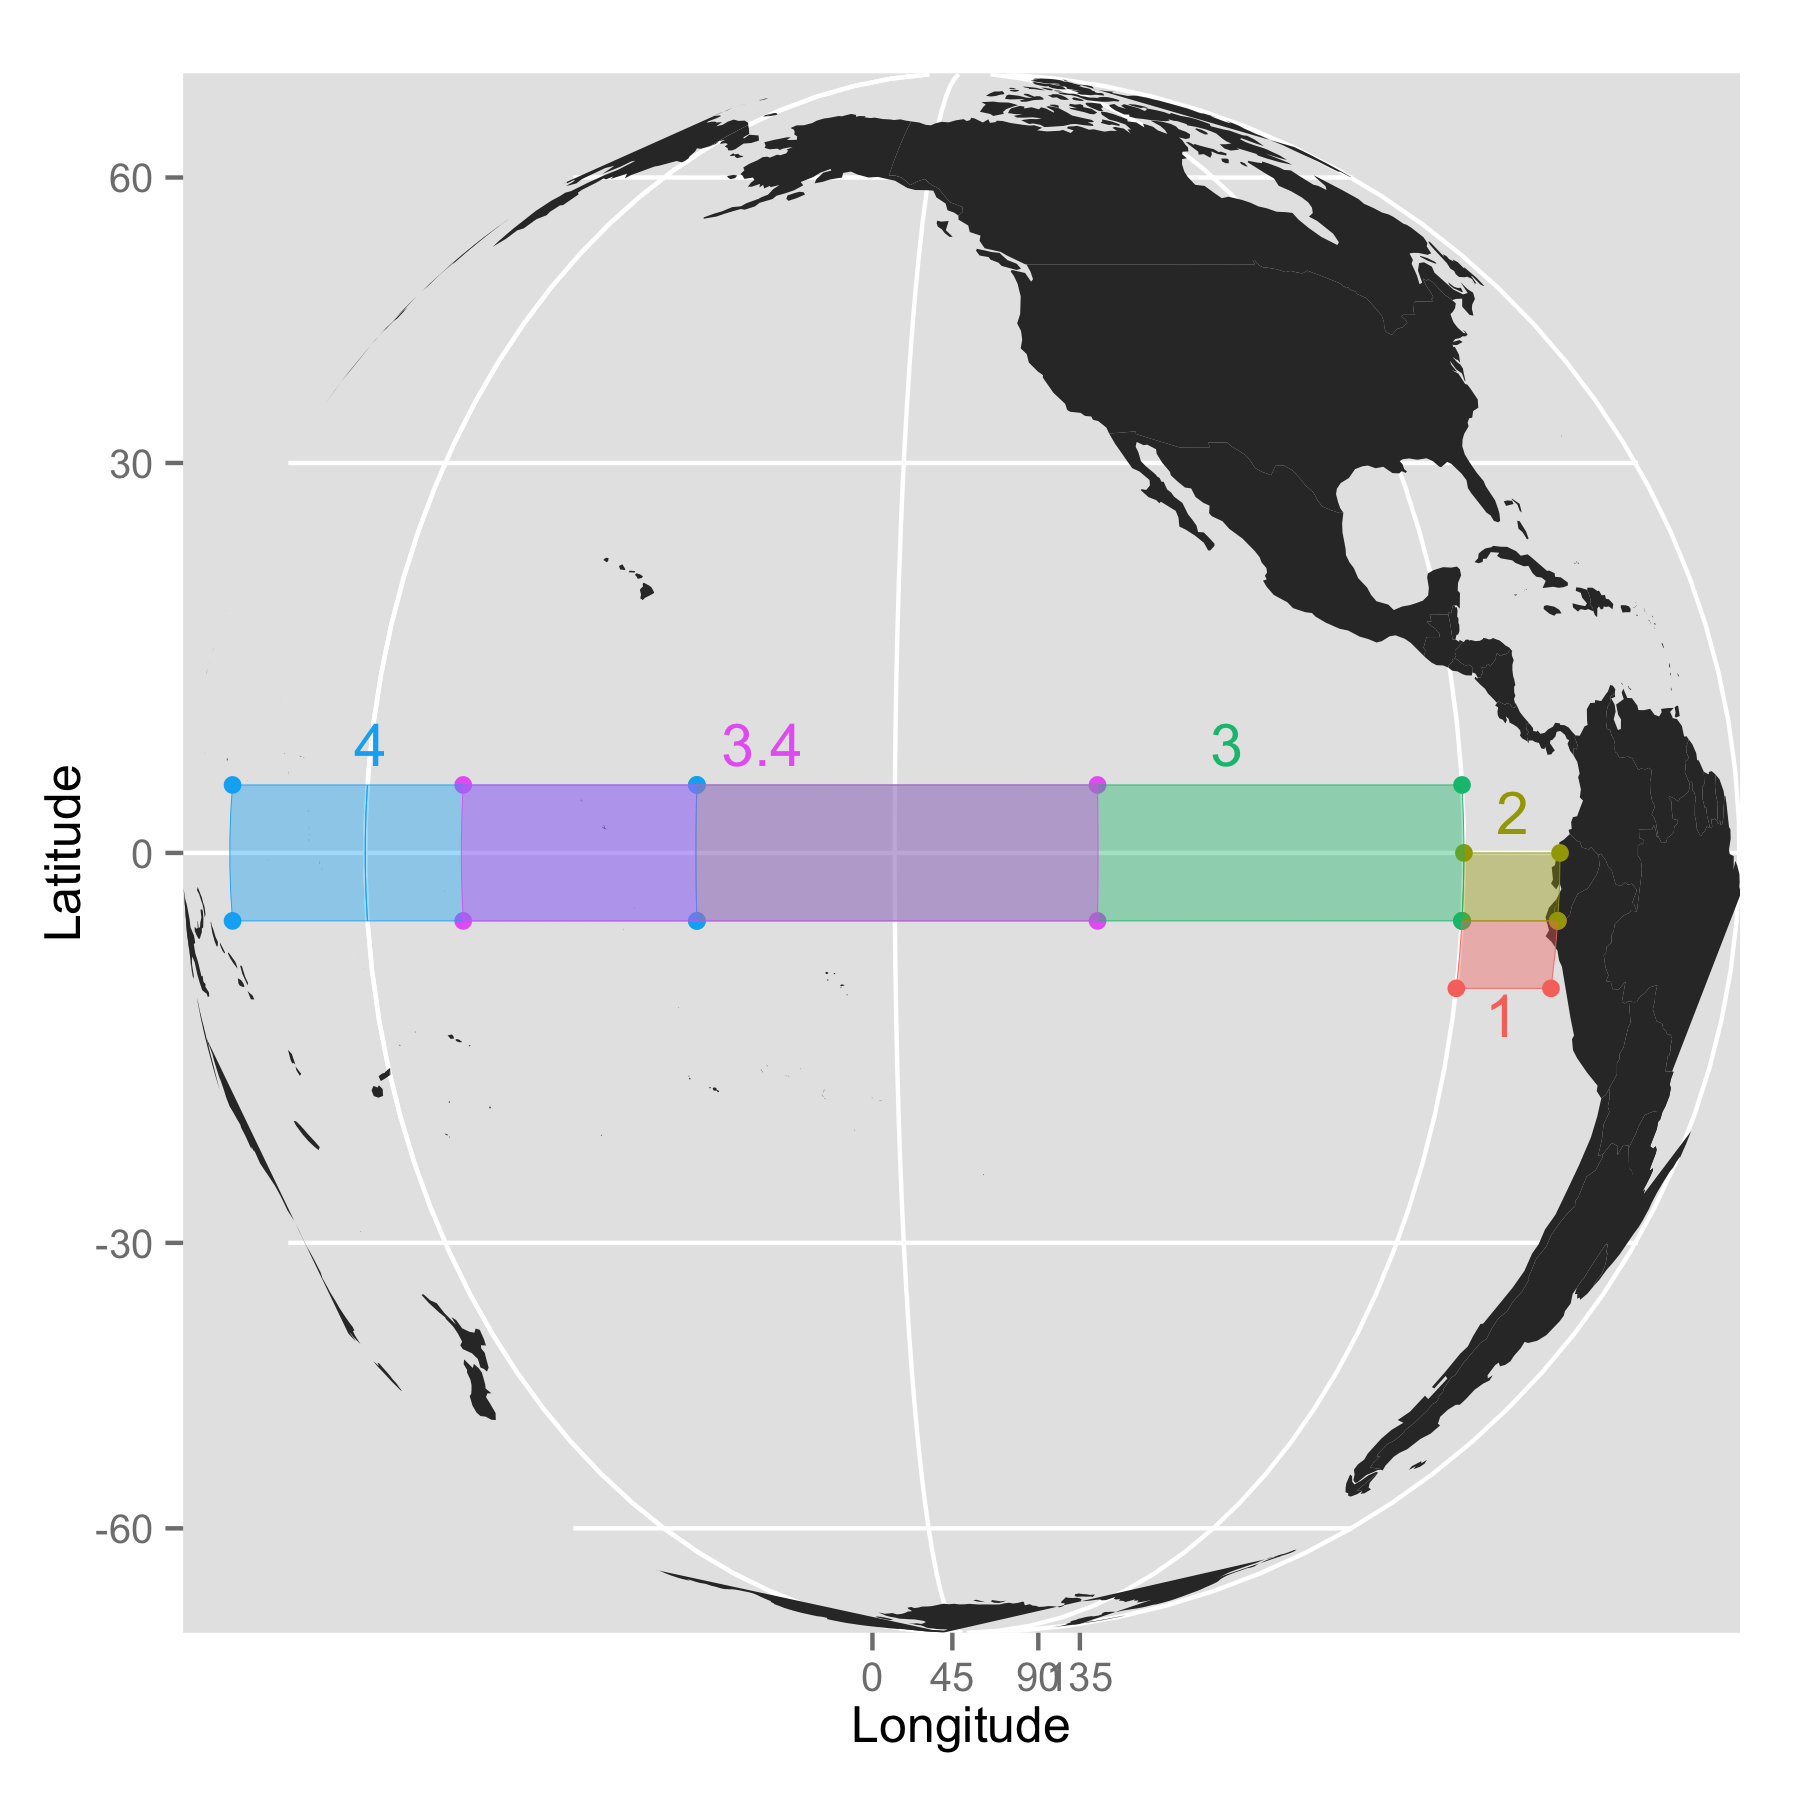
\includegraphics[width=\linewidth]{img/region_map.png}
  \caption{NOAA's \text{Ni\~no} SST regions}
  \label{fig:ninoareas}
\end{figure}

That link between high SSTs and rainfall is dramatic. In figure
\ref{fig:pptInPiura} \emph{need to reproduce} we see that rainfall in
northern Peru during the last severe El \text{Ni\~no} in 1998 was 40
times normal for January to May (Skees and Murphy 2009). This event
caused widescale internal displacement of people, loss of life,
increases water-born illnesses, disruptions to markets and supply
chains, and destruction of personal property and critical infrastructure
(Rosenzweig and Hillel 2008). There were similarly alarming impacts from
the 1983 El \text{Ni\~no} which was also linked to the economic collapse
of the country's fishing industry (Glantz, Katz, and Nicholls 1991;
Aranda 2009).

\begin{figure}
  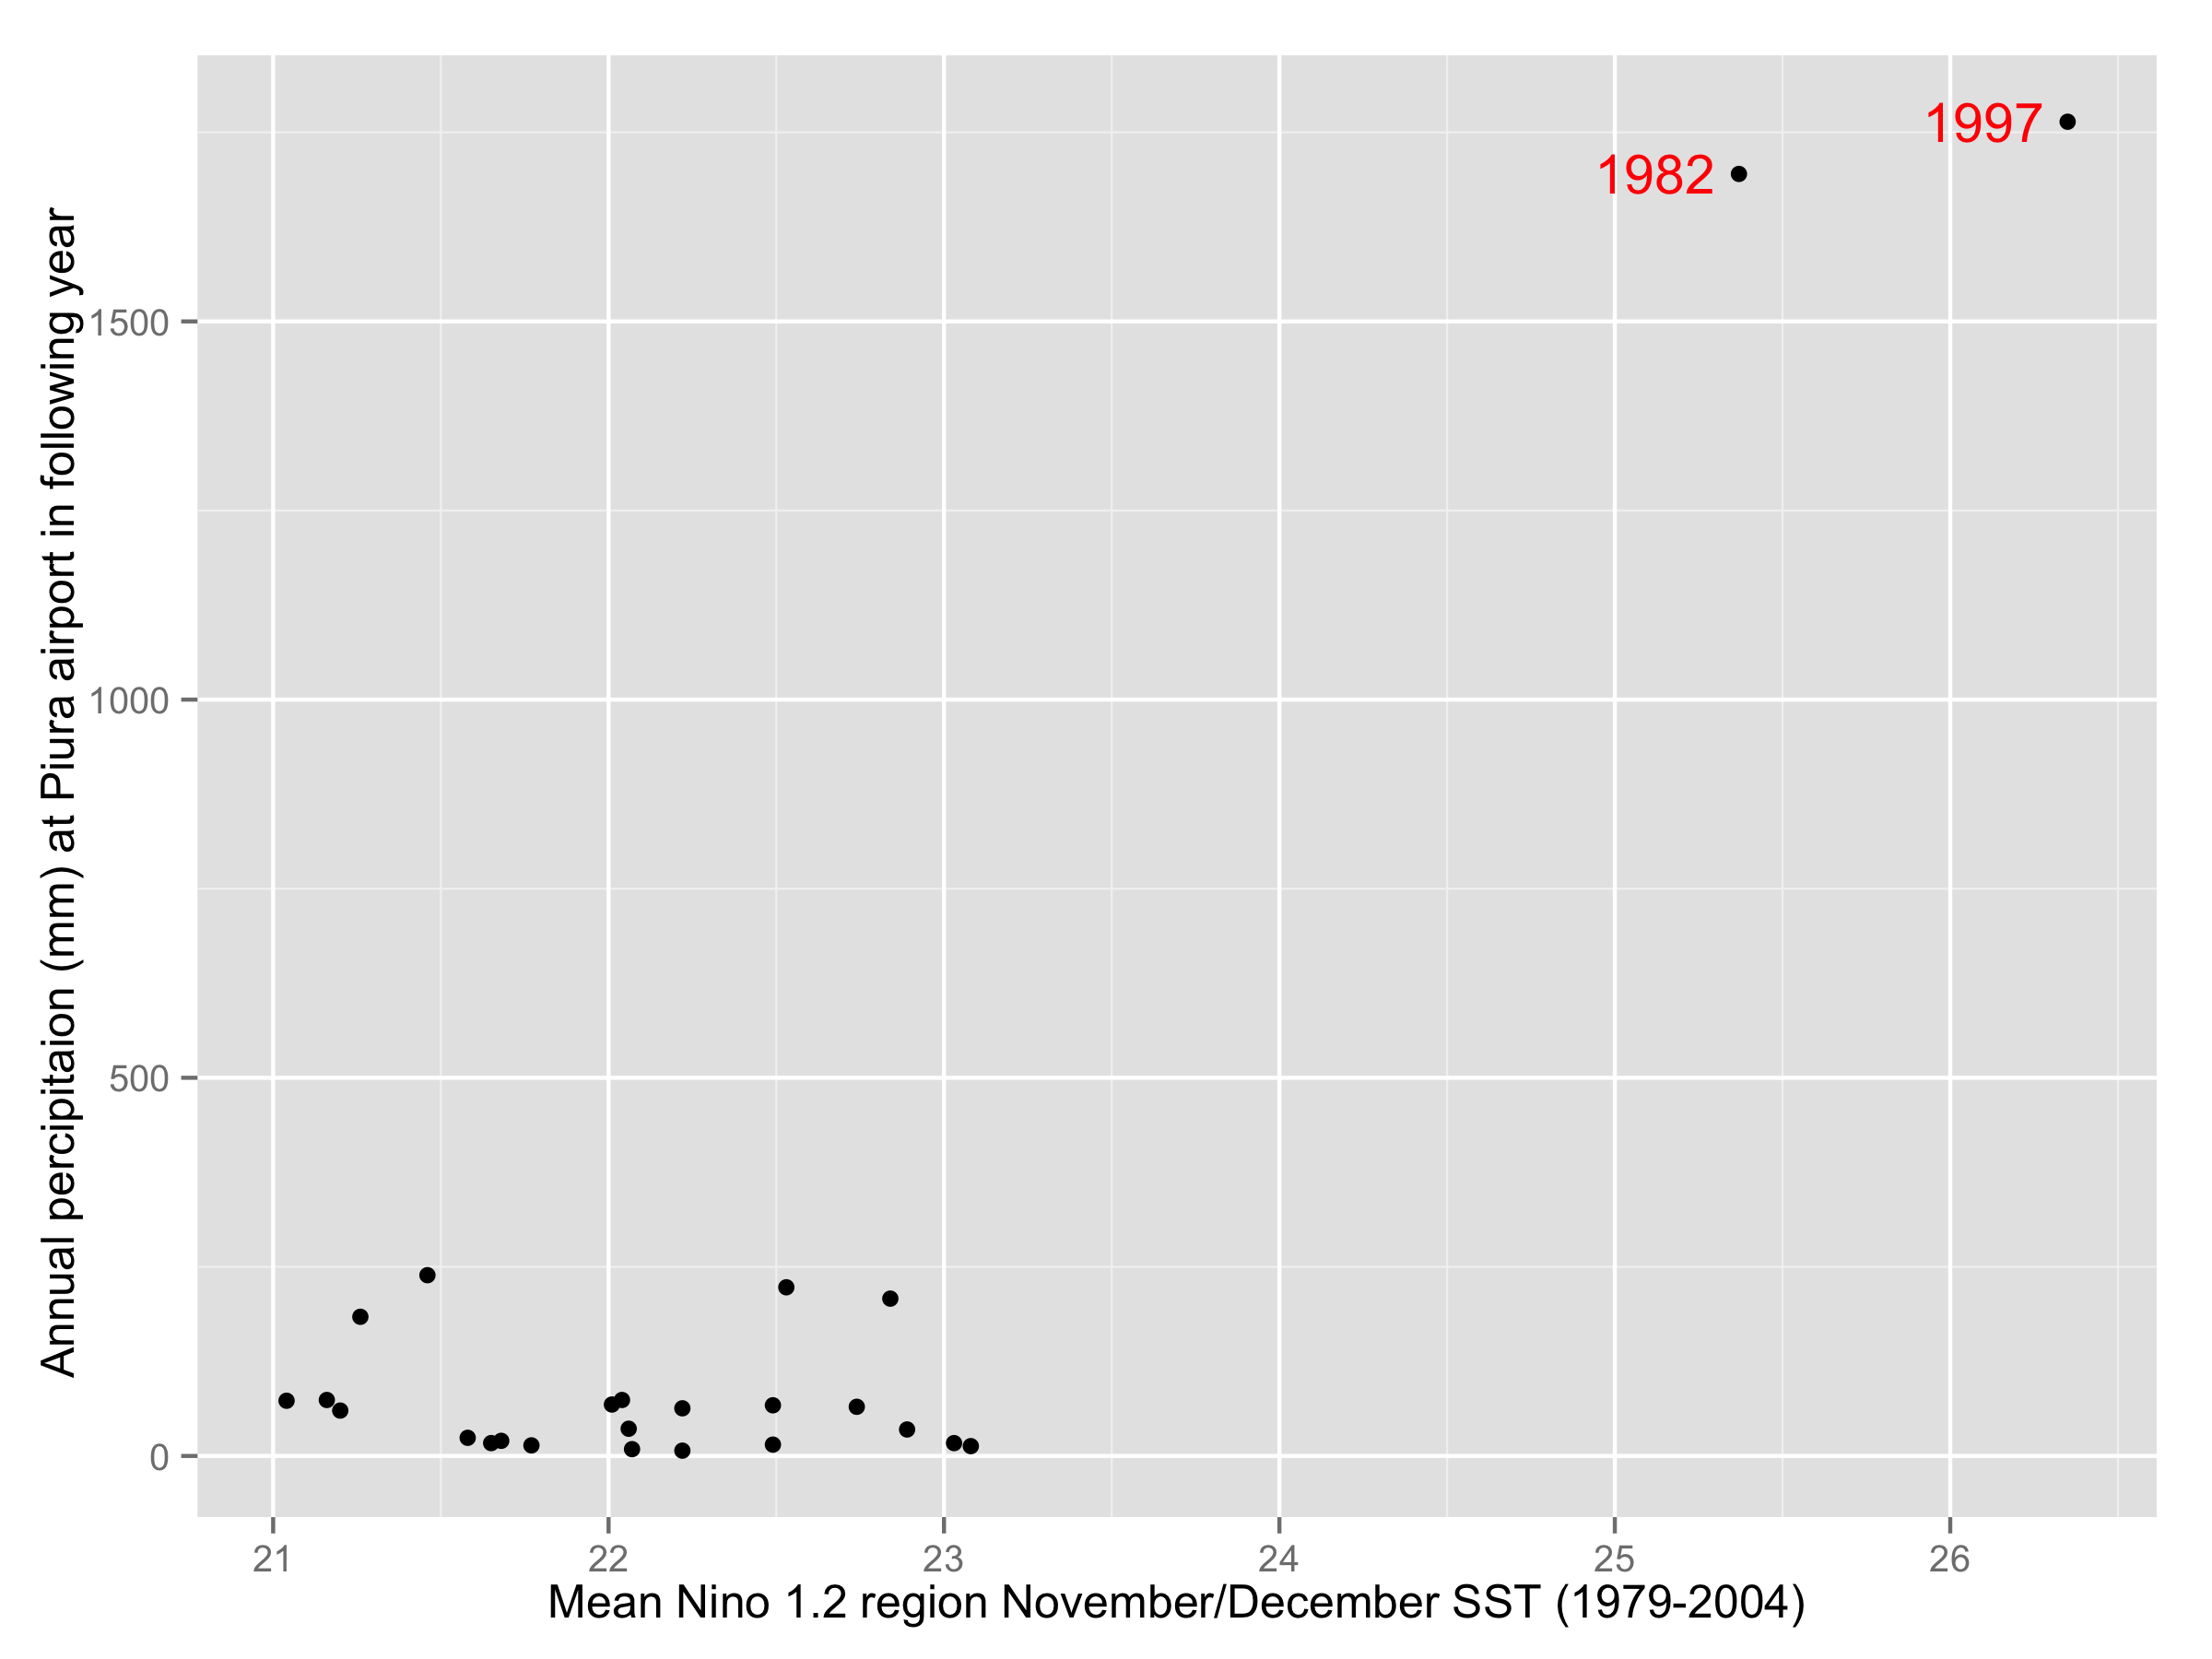
\includegraphics[width=\linewidth]{img/piuraPptScatter.png}
  \caption{Mean Nino 1.2 region November/December SST (1979-2004) vs. annual percipitaion (mm) at Piura airport in following year (data from Mario Miranda and Jerry Skees)}
  \label{fig:pptInPiura}
\end{figure}

Importantly from the standpoint of a hedger evaluating basis risk, both
of those extreme anomaly years stand out in \text{Ni\~no} SST time
series. The spikes in that index correspond so well to the years
popularly associated with catastrophic El \text{Ni\~no}, that most
hedgers expressed satisfaction that they would receive some payment
should another catastrophic El \text{Ni\~no} occur.

\subsection{Spatially correlated risk}\label{spatially-correlated-risk}

Car accidents provide a simple example of a \emph{pooled risk}.Everyday
that a driver does not get into an accident, they are implicitly paying
car insurance premiums that go into a pool used to pay the claims of the
few drivers that did get into an accident that day. Historically, the
price of insurance on such pooled risks is strongly linked to underlying
expected loss (Cummins and Tennyson 1992). This leaves little room for
efficiency improvement through trading.

However, spatially correlated risks like El \text{Ni\~no} cannot be
pooled (Skees, Hartell, and Murphy 2007). The vast majority of Peruvians
facing El \text{Ni\~no} risk experience that risk at the same time -
every year will either bring a catastrophic El \text{Ni\~no}, against
which they would like protection, or it will not.

Within the world of insurance, spatially correlated risk tend to pass to
reinsurance companies - companies who have enough capital to payout huge
claims at a moments notice. These companies ostensibly pool their risks
across the globe - balancing, for example, US hurricane risk in a
portfolio with Turkish earthquake risk. However, in practice, their
portfolios are highly concentrated and their business model involves
accepting catastrophic risk in exchange expected profits that are
multiples of the underlying risk. (Estimates of industry-wide pricing to
risk ratios are avaliable through periodic publications by brokers such
as Schultz (2012), Ursano (2013), and Swiss Re (2012). One plausible
explanation of persistently high reinsurance prices is that the supply
of large capital reserves required in reinsurance are constrained (K.A.
Froot 2001).

\begin{verbatim}
                                                                                                                                                                                                                                                                                                                                                                                                                                                                                                                                      Industry experts have long believed that the unpoolable risk in reinsurance markets could be managed more efficiently in traded markets, where groups of speculators could replace large reinsurers and competition among those speculators would drive prices down [@sandor2012]. Almost two decades after the first experiments moving reinsurance risk to traded markets, that _convergence_ between reinsurance and broader financial markets appears to be underway, with reinsurers reporting that recent falls in prices have been driven by outside pools of risk capital [@schultz2012; @willis201ils; @swiss2012update]. From the standpoint of ENSO and other teleconnection risks, this convergence suggests that traded markets are a viable and potentially efficient avenue for managing risks that might otherwise go to reinsurance markets.
\end{verbatim}

\subsection{Cyclical risk}\label{cyclical-risk}

El \text{Ni\~no}/La \text{Ni\~na} emerge in the latter months of the
calendar year. That annual cycle allowed GlobalAgRisk to construct an
innovative insurance that offeres payouts in advanace of the floods that
are the chief concern for at-risk Peruvians. However, ENSO's annual
cycle also poses informational challenges to any potential ENSO risk
markets.

High SSTs in specific months define El \text{Ni\~no}/La \text{Ni\~na}.
But those high SSTs precede the rains they cause. GlobalAgRisk's El
\text{Ni\~no} insurance takes advantage of this lag. It makes payments
using November and December ocean temperatures, which predate the severe
rains and flooding that have historically begun in late January/early
February. That lag means the insurance payments could be used for loss
mitigation and adaptation. That innovative feature is understandably
attractive to buyers (Khalil et al. 2007). However, it rests on the fact
that ENSO risk can be forecast, which itself is problematic for
speculators.

Sustained Pacific temperature anomalies build up over months, with the
cycle of build-up generally reset at the end of the Northern Hemisphere
winter. Each year starting in March, current temperature readings that
are warmer or colder than normal SSTs provide probabilistic information
about the temperatures that we will see in the critical months later in
the ENSO season that define El \text{Ni\~no}/La \text{Ni\~na}. The
signal provided by those current SSTs strengthens throughout the year,
such that forecasts are less reliable in April than they are in June
(Clarke 2008).

That creates a problem for speculators in ENSO risk. If buyers are
particularly skilled at forecasting SSTs, they may buy ENSO protection
only in those years when they are likely to enjoy a payout. That type of
herding behavior is known in insurance markets as adverse selection and
(re)insurance companies try to avoid it by setting their \emph{sales
closing date}, the last date on which buyers can commit to an insurance
arrangement, well in advance of the time when actionable forecasts
emerge.In other words, (re)insurers refuse to participate in risk trades
where they believe it is necessary to condition historical prices on
current forecasts.

When El \text{Ni\~no} insurance first came on the market in Peru, the
sales closing date was set in March. While this was near the
\emph{spring predictive barrier} in the ENSO cycle, the reinsurer
backing the product was not satisfied that the sales closing date
preceded all actionable forecasts. In subsequent seasons, the sales
closing date for GlobalAgRisk's insurance was pushed back to January,
almost a full year before the period of coverage (G. Cavanaugh, Collier,
and Skees 2010).

This schedule avoids the adverse selection problems created by El
\text{Ni\~no} forecasts, but it also limits participation in this
market. For some firms, the high opportunity cost of purchasing
insurance so far in advance is too great. For others, the rigid and
long-dated sales parameters conflict with existing budget cycles. Those
problems will only grow over time as forecasting likely continues to
improve, requiring earlier and earlier sales closing dates.

Multi-year insurance agreements might alleviate the threat of adverse
selection linked to ENSO forecasts, at least for the latter years of
those contracts since even ambitious forecasts forecasts rarely claim to
extend beyond a year. They will also smooth insurance demand in a market
where many policyholders might fail to renew their policies in the year
(or several years) following a severe event, believing that neutral or
La \text{Ni\~na} events naturally follow El \text{Ni\~no}. That belief
is not well founded in historic records, but it is common enough to
produce fluctuations in demand that might discourage insurers and
brokers, who build their business on automatic renewals.

But multi-year contracts only exacerbate the opportunity cost problem
facing insurance buyers. Not only will they require buyers to make a
decision on the insurance and lock up premiums ahead of forecasts for
the front year of the contract, but they will also have to lock up
premiums for the latter years of the contract. Moreover, reinsurance and
related markets rarely offer standardized risk transfer agreements that
extend beyond a year. (Some industry experts have reported that
reinsurers have reluctantly begun to offer multi-year policies in
response to recent competitive pressures (Evans 2013). However,
catastrophe bonds, which remain among the longer dated relevant contract
types generally extend out three years, and only rarely more than five
(Kurtov 2010).)

On traded markets, prices for protection move to reflect new forecast
information as it becomes available. With such dynamic pricing of ENSO
risk, buyers could enter and exist hedges at their convenience assuming
that most of the private information available to the market has already
been incorporated into prices. If any trader identifies a mis-pricing
with high confidence, they can use leverage to magnify the returns to
their private information. That type of aggressive speculation should
theoretically limit the scale of information asymmetries faced by future
hedgers.

To be sure, adverse selection can undermine liquidity in traded markets,
just as in insurance markets (Copeland and Galai 1983; Glosten and
Milgrom 1985; Kyle 1985; Leland 1992). However, traded markets routinely
incorporate the type of probabilistic information contained in ENSO
forecasts without incident. While it is theoretically possible for
insurance companies to offer dynamic pricing of risks similar to a
traded market, the firm offering such prices would bear all of the
adverse selection risk in that market.

\subsection{Forecasts have social
value}\label{forecasts-have-social-value}

When first presented with GlobalAgRisk's El \text{Ni\~no} protection,
Peruvians regulators debated whether the product should be regulated as
a derivative or as an insurance. Quickly, they decided that the product
should be an insurance because Peruvians had an \emph{insurable
interest} in the proposed policies - they routinely saw forecasts of
ENSO SST index anomalies in the media and incurred costs preparing for
impending disaster based on those forecasts. So, even before formal El
\text{Ni\~no} protection was available, forecasts of indexes of the risk
were demonstrating clear social value by driving economic decisions.

Like any risk trade, insurance prices could to contribute to the process
of disseminating actionable forecast information. But, as discussed
above, reinsurance companies rarely offer conditional pricing on risks
like ENSO that emerge over time. Even if they did insurance policies
often include provisions baring purchasers of protection from revealing
the price they received. So many industry practices limit the
contribution of insurance transactions to public forecast information.

By contrast, traded markets have a long history not just of reacting to
new information, like ENSO forecasts, but anticipating and synthesizing
those forecasts into a single reliable signal that can guide economic
decision making. Looking at a market with clear ties to teleconnection
risk, Chincarini (2011) found that weather derivatives prices, even for
thinly traded contracts, provide a reliable benchmarks for prediction.
Roll (1984) identifies instances when orange juice concentrate futures
have price movements anticipate severe weather forecasts before they
were released by the U.S. National Weather Service.

In the case of ENSO, prices from traded markets will be valuable
precisely because there is so much publicly available forecasting.
Hedgers find it difficult to process competing forecasts in the absence
of definitive baseline reference points, like the prices from markets.
In any given month, some NMS predict looming catastrophe while others
tell hedgers not to worry. Figure \ref{fig:IRIENSOconsensusSpread}
provides a sense of the range of forecasts throughout 2012, a year in
which conditions were ultimately normal. In early 2012 some models
predicted historically strong El \text{Ni\~no} while others suggested a
light La \text{Ni\~na}.

\begin{figure}
  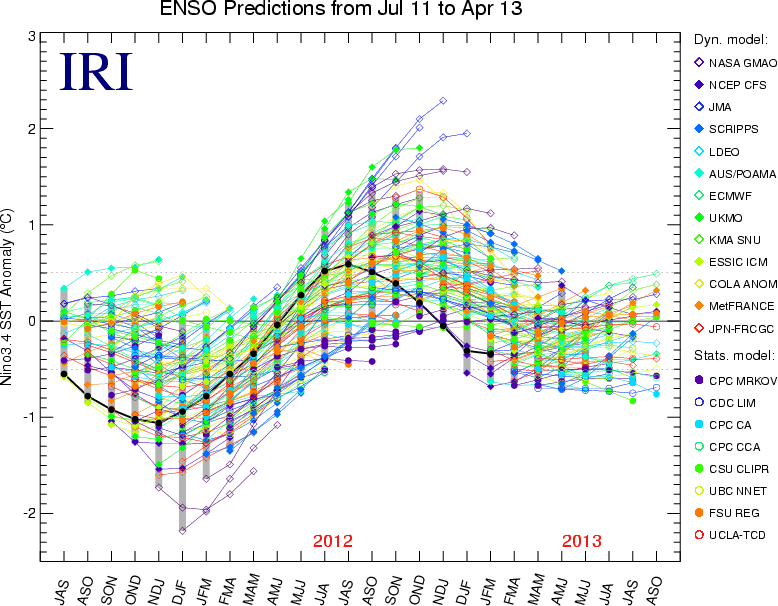
\includegraphics[width=\linewidth]{img/all_forecasts_IRI_04_2013.png}
  \caption{Forecasts of ENSO index anomalies between July 2011 and April 2013 compiled by Columbia University's International Research Institute for Climate and Society \url{http://portal.iri.columbia.edu/}}
  \label{fig:IRIENSOconsensusSpread}
\end{figure}

Researchers are comfortable harnessing that disagreement among models to
provide ensemble forecasts (Coelho et al. 2004; Luo, Wood, and Pan
2007). But, Peruvian hedgers repeatedly expressed confusion linked to
the proliferation of ENSO forecasts in meetings with GlobalAgRisk. In
particular, some hedgers came to mistaken conclusion that relatively
mild years for \text{Ni\~no} SST were actually extreme El \text{Ni\~no}
years based on individual forecasts. That confusion about past ENSO
forecast may have reprocussions for future preparedness. Gladwin and
Peacock (1997) found that individual who survived a hurricane were
actually less likely to evacuate when threatened by subsequent large
storms.

In the context of proliferating forecasts, a single concensus forecast
(in the form of a price for protection) may be particularly valuable to
at-risk individuals. Given the link between ENSO and the wider process
of global climate change, forecasts from ENSO markets may also provide
valuable, if indirect, forecasts for global weather patterns beyond the
regions traditionally associated with ENSO.

\subsection{Offsetting pools of risk}\label{offsetting-pools-of-risk}

Early work on ENSO risk management has focused on Peru. But,
teleconnections, like ENSO, inherently link disparate groups of hedgers
across the globe. Where Peruvians see El \text{Ni\~no} anomalies as
harbingers of disaster, American insurers see them as an indicator of
strong underwriting profits thanks to a decreased likelihood of major
Atlantic hurricanes (Klotzbach 2011). Ropelewski and Halpert (1987) and
Ropelewski and Halpert (1989), seminal academic articles at the heart of
our current understanding of ENSO, identify many far-flung regions (19
for El \text{Ni\~no} and 15 for La \text{Ni\~na}) where precipitation
has a statistically significant link to the ENSO cycle.

In theory, the diversity of ENSO's impacts across time and space means
that hedgers with offsetting risk profiles could directly trade risk
with one another. Relative to a \emph{one-sided} market, like
reinsurance, where a speculator (reinsurer) sets a price above expected
loss that a hedger can take or leave, direct trades between hedgers
would improve social welfare in the short-run.

In a direct trade, each hedger is willing to transact with little or no
expected profit because the trade would improve their risk profile. Such
\emph{two-sided} markets, where buyers and sellers simultaneously
negotiate, would also allow firms with strong forecasts of ENSO to enter
the market as buyers or sellers, depending on prevailing prices. Hence,
a two-sided ENSO market would have two important short-run advantages
realtive to simple reinsurance:

\begin{itemize}
\itemsep1pt\parskip0pt\parsep0pt
\item
  hedgers could cost-effectivly achieve a given risk profile;
\item
  natrual hedgers and speculators could both contribute to price
  discovery.
\end{itemize}

While these advantages would not persist in a perfectly competetive
marketplace, market frictions are a long-standing empricial reality in
reinsurance. Reinsurers have enjoyed high expected profits for decades
and the distinction between reinsurance buyer and seller is enforced
through regulation (K. Froot 1999).

To be sure, a one-sided market is perfectly appropriate for some types
of risks. For example, hedging interest in earthquake risk is naturally
\emph{unbalanced}. There is no large group of firms that benefits from
an earthquake and would consequently be willing to accept earthquake
losses at no expected profit. A two-sided market in eaerthquake risk
would quickly reduce to a one-sided market, with all hedgers buying
protection from speculators. However, teleconnection risk is natually
balanced. That means that its markets would enjoy a rare and valuable
advantage as they attempt to establish liquidity in a two-sided format
(e.g.~derivatives, traded securities, etc.) (Gray 1978; Tashjian 1995)
which in turn promises low-cost and informationally efficient trading in
the short-run.

\subsection{There are few simple, reliable proxies for ENSO
risk}\label{there-are-few-simple-reliable-proxies-for-enso-risk}

The last important quality to note about ENSO risk is that it is not a
simple combination of other common risks nor is it a risk that can be
recreated physically. The ability to recreate a risk (physically or
statistically) is a prerequisite for arbitrage pricing formulas. Those
formulas can be helpful to a new market looking to reach sustainable
liquidity because they provide a stable reference price for
transactions. However, easy opportunities for arbitrage can also obviate
the need for a dedicated risk markets. Why hedge on a new illiquid
market when an existing liquid market offers very similar hedges?

Taken togeather, these factors suggest that:

\begin{itemize}
\itemsep1pt\parskip0pt\parsep0pt
\item
  There is an opportunity for ENSO and other teleconnection risk markets
  because they would not be redundant; however,
\item
  Taking advantage of that opportunity will require simple pricing
  huristics that can take the place of an arbitrage formula.
\end{itemize}

We cannot store sea surface temperates, atmospheric patterns, or any of
the defining charateristics of regional climate anomalies. This rules
out physical arbitrage for teleconnection risk. It is also difficult to
find strong statistical \emph{cross-hedges} for teleconnect risks. For
example, industry experts may note that ENSO is linked to poor growing
conditions for cocoa in West Africa and high summer temperatures in
Houston (Agbroko 2012; Electric Reliability Council of Texas (ERCOT)
2014). They may subsequently use ENSO information to trade on cocoa
futures and Texas electricity markets. However, it would be very
difficult to use a basket of cocoa and electricity to reconstruct an
index of ENSO.

The absence of arbitrage, suggests first that ENSO risk should be
managed on dedicated markets. Second, it also suggests the need for
simple and reliable reference prices based on historical information to
catalyze risk trades. In many markets, arbitrage pricing formulas help
catalyze trades by lowering the analytical barriers to entry and
limiting the scale of information asymmetries (Scholes 1998). Traders
place a particular emphasis on arbitrage based reference prices because
they tend to have strong theoretical underpinnings and the prices they
produce can be enforced through simple trading strategies.

Nevertheless, in circumstances where there is no reliable arbitrage,
pricing frameworks based purely on historical data are the best
available alternative and are often quite effective at approximating
arbitrage pricing and thereby eliminating gross inefficiencies in a
market (Haug and Taleb 2011). In the latter sections of this article, we
present such a framework.

\section{Pricing direct climate risk}\label{pricing-direct-climate-risk}

The remainder of this article focuses on the data and decision-making
hurdles surrounding the launch of traded risk markets on teleconnection
index risk.

Again we focus on ENSO, for which we:

\begin{itemize}
\itemsep1pt\parskip0pt\parsep0pt
\item
  identify NOAA's monthly SST from the \text{Ni\~no} 3.4 region compiled
  using the ERSST 3b methodology as the most promising of the candidate
  ENSO SST indexes for contract settlement;
\item
  approximate a fair price for risk transfer conditional on available
  forecasts when no arbitrage is available; and,
\item
  use prices and historical data to identify key times in the ENSO cycle
  in which trading is likely to concentrate.
\end{itemize}

Having identified two-sided markets as an end goal, the remainder of
this article focuses on practical concerns regarding the launch of those
markets. This analysis is not only necessary to support sustained ENSO
risk trading, but will be important for the related climate-linked
markets that follow in its wake.

\section{Choosing a index}\label{choosing-a-index}

There are multiple SST datasets that could settle ENSO risk transfer
contracts. In this section we explain why NOAA's monthly SST from the
\text{Ni\~no} 3.4 region compiled using the ERSST 3b methodology is a
particularly strong candidate to settle traded risk contracts.

We arrive at this conclusion after considering the a series of questions
that distinguish NOAA's SST datasets from one another:

\begin{itemize}
\itemsep1pt\parskip0pt\parsep0pt
\item
  Which methodology does it use?
\item
  Which region does it cover?
\item
  In what form are the SSTs presented?

  \begin{itemize}
  \itemsep1pt\parskip0pt\parsep0pt
  \item
    As absolute degrees or anomalies?
  \item
    As individual monthly measures or as values smoothed across rolling
    windows?
  \end{itemize}
\end{itemize}

\subsection{Choosing a methodology}\label{choosing-a-methodology}

NOAA publishes two primary sea surface temperate indexes. Figure
\ref{fig:baeslinesOIER} provides the monthly values that NOAA uses to
calibrate anomalies in each. NOAA's Extended Reconstructed Sea Surface
Temperature Index (ERSST) dataset provides a longer record compiled
using in-situ buoy measurement. NOAA's satellite-based Optimum
Interpolation Sea Surface Temperature Index (OISST) offers finer
resolution. While they are compiled using distinct methodologies, both
indexes agree when identifying extreme El \text{Ni\~no}/La \text{Ni\~na}
events. Given its longer record, the conceptual simplicity of in-situ
data collection, and the documented bias of the OISST methodology toward
colder temperatures, we favor the use of ERSST as the basis of financial
contracts. However, the cost and reliability of ERSST buoys may guide
NMS toward greater reliance on OISST. In either case, the financial
considerations outline here remain the same.

\begin{figure}[!htbp]
\begin{center}
  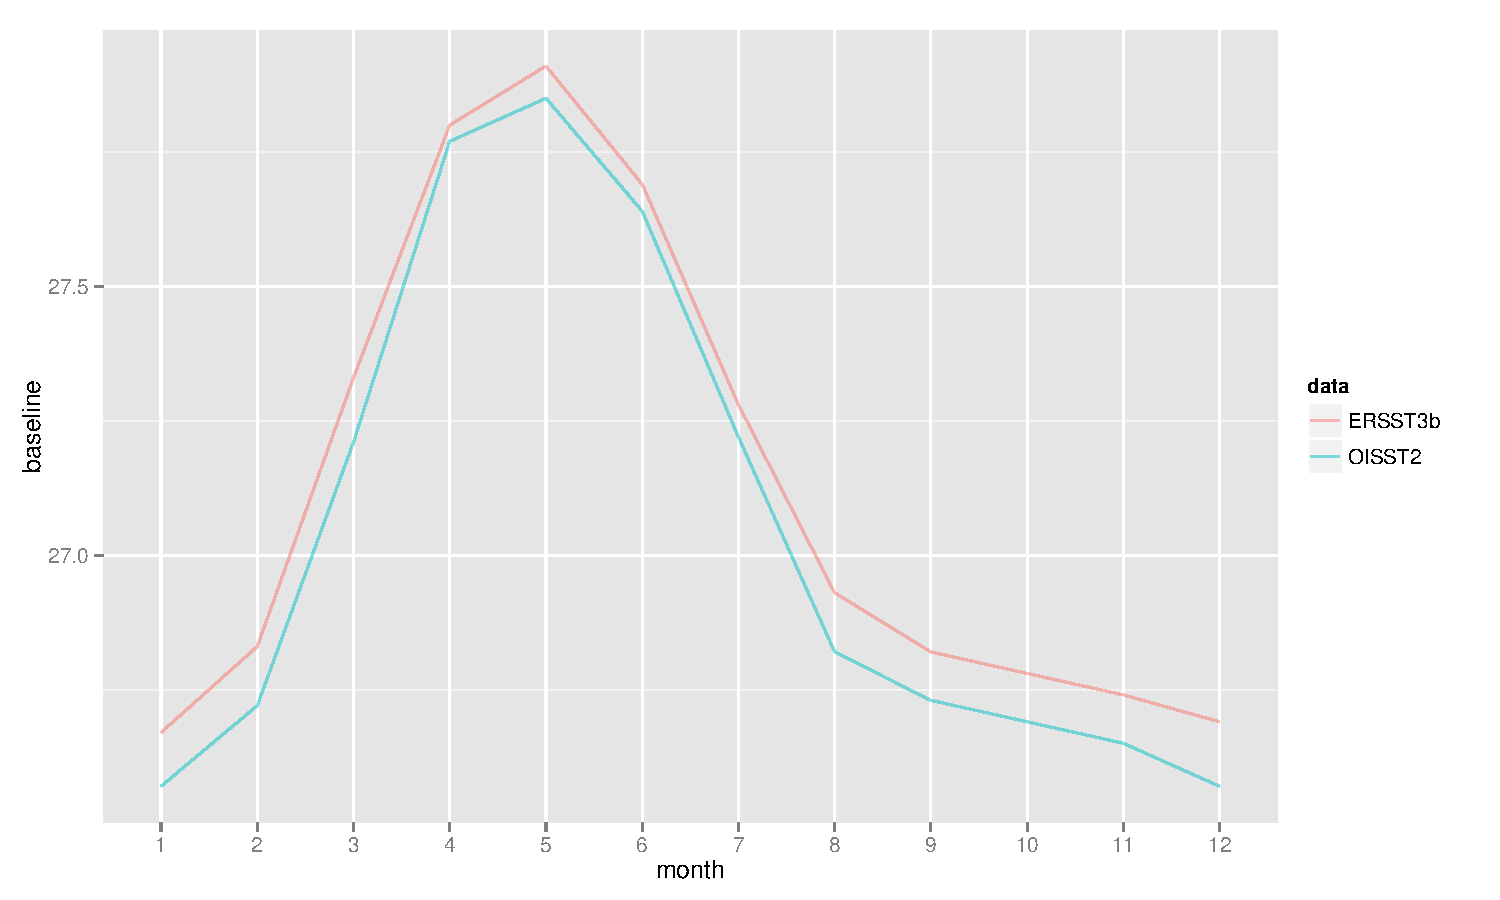
\includegraphics[width=\linewidth]{img/CompareOISSTandERRSTbaselines.pdf}
  \caption{Comparing OISST and ERSST monthly baselines}
   \label{fig:baeslinesOIER}
   \end{center}
\end{figure}

The key factor distinguishing ERSST from OISST is the use of in-situ and
satellite data. ERSST exclusively uses in-situ measurement, primarily
that consists of temperature readings taken by a network of buoys
throughout the Pacific (which are now communicated via satellite) (Smith
and Reynolds 2004; Smith and Reynolds 2003; Smith et al. 2008). Monthly
anomalies in the ERSST version 3b index are measured relative to a
1971-2000 base period with a resolution of two degrees across the four
ENSO regions (Xue, Smith, and Reynolds 2003). While the primary index
record that NOAA posts to its websites goes back to 1950, monthly ERSST
data are available from 1854 on.

OISST, currently at version 2, combines in-situ SST measurements,
daytime and nighttime satellite data readings, and data from sea ice
cover simulations. The satellite-measured data, whose collection began
in the early 1980s, is adjusted statistically for natural sources of
bias, like cloud cover and atmospheric water vapor (Reynolds et al.
2002; Reynolds and Smith 1994; Reynolds and Marsico 1993; R. W. Reynolds
1988).

Finance professionals require reliability, simplicity, and prefer a long
track record for their settlement indexes. Neither ERSST nor OISST has a
clear advantage across all three dimensions.

ERSST relies on data that is relatively simple for non-experts to grasp
- buoys take temperature readings at regular intervals and relay that
information via satellite. Indeed, that is the reason that the
GlobalAgRisk team used ERSST data to price its El \text{Ni\~no}
insurance. By contrast, OISST combines data from multiple sources in a
procedure that requires some advanced climate and statistical knowledge
to parse.

However, ERSST's buoys are subject to a higher risk of physical damage
than the remote measurement tools used for OISST. When a buoy is
offline, NOAA uses statistical techniques to infer data from surrounding
buoys. This means that in practice the integrity of ERSST's underlying
data may be lower and the index may ultimately rely equally on
statistical procedures obscure to new hedgers.

The reason that we believe that ERSST is ultimately a better index for
financial contract settlement is its age. ERSST simply offers a longer
time series for price analysis. Using ERSST, gives practitioners almost
thirty-five additional historical data points for any given month. Those
extra data points provide everyone involved with a great deal more
confidence in their pricing models.

\subsection{Choosing a region}\label{choosing-a-region}

\text{Ni\~no} 1.2 is the best predictor of catastrophic flooding in Peru
and Ecuador consequently it was the basis for the existing El
\text{Ni\~no}'s insurance (Khalil et al. 2007). However, NMS generally
mark global ENSO anomalies using the \text{Ni\~no} 3.4 region, which
stretches across the central Pacific (Barnston, Chelliah, and Goldenberg
1997). Both regions, \text{Ni\~no} 1.2 and the \text{Ni\~no} 3.4, have a
very high correlation during extreme anomalies. But \text{Ni\~no} 3.4 is
generally considered a better proxy for the worldwide teleconnections
associated with ENSO. In particular, it does a better job capturing ENSO
anomalies with distinct geographic signatures. During the 1972/1973 El
\text{Ni\~no}, for example, most of the sea-surface temperature warming
occurred in the central Pacific, closer to the \text{Ni\~no} 3.4 region.
El \text{Ni\~no} events focused on the Central Pacific are also called
\emph{Modoki} \text{Ni\~no}s and can have large global impacts (Ashok et
al. 2007).

\subsection{Choosing a format}\label{choosing-a-format}

After selecting a settlement index, market innovators must also choose
the format in which settlement numbers will be presented to traders. In
the case of ENSO, that choice centers on the question of whether to use:

\begin{itemize}
\itemsep1pt\parskip0pt\parsep0pt
\item
  Anomalies (degree Celsius departures from monthly averages) or
  absolute degrees Celsius; and,
\item
  Simple monthly values or moving averages, with for example, a three
  month window.
\end{itemize}

It is not immediately clear whether anomalies or absolute degrees offer
a better base for financial contracts. Early potential market
participants interviewed in (Grant Cavanaugh 2013) were split or
indifferent on this question.

The work here is presented in terms of absolute values to mirror the
format of the existing El \text{Ni\~no} insurance. However, most major
meteorological organizations define El \text{Ni\~no}/La \text{Ni\~na}
events in terms of persistent monthly anomalies. Indeed, many forecasts
of SSTs (like those from the ABM and IRI) are only provided in terms of
anomalies. So, early traders may feel more comfortable thinking in terms
of anomalies.

The primary disadvantage of anomalies is that they can obscure changes
over time because they are based on averages from a rolling window (e.g,
using data from the previous 20 years). Those baselines have been, and
will continue to be, subject to revision as underlying SSTs drift over
time. This means, for example, that a 2 degree positive anomaly in
October relative to the current baseline may and likely will be
different in absolute temperature than a 2 degree positive anomaly in
October twenty years from now.

That shift in baseline SSTs, likely driven by global climate change, is
one of the areas where market forecasts could inform public policy. It
is marginally obscured by using anomalies with changing baselines. For
example, if climate change increases the mean of ocean temperatures, the
terms of a relative contract would also adjust. So, trading in 2016 and
2030 might both center on a one degree anomaly, but the baseline
defining that anomaly might change. To a naive observer, this might look
like a twenty year period in which traders did not price in any change
in the underlying climate. Using absolute temperatures, traders could
easily express theories about the long-term trends in the index in a way
that is simple and clear to uninformed observers.

In either case, the choice between anomalies and absolute units is one
of convenience. It is not integral to the success of the market. Many
weather derivative routinely use annually revised baselines.

By contrast, the choice between using individual monthly values and
multi-month averages is more straight-forward. Multi-month averaged
indexes are commonly used by NMS to define ENSO. (GlobalAgRisk's
existing insurance settles on a multi-month average.) But single month
contracts would offer traders greater flexibility as they attempt to
profit from fine-resolution forecasts. If there were traded markets on
monthly values, it would be trivial to combine them and create a
positions that mirror multi-month indexes.

\section{Developing a prototypical
contract}\label{developing-a-prototypical-contract}

Given a target index, we now begin the process of pricing contracts on
that index built around the needs of hedgers. That process involves:

\begin{itemize}
\itemsep1pt\parskip0pt\parsep0pt
\item
  Choosing a pricing function to convert index values into financial
  obligations;
\item
  Running historical values through that pricing function, and
\item
  Fitting a distribution to historical values to generate prices that
  reflect the underlying statistical process of ENSO.
\end{itemize}

Based on the recommendation of Dr.~Andrew Watkins of the Australian
Bureau of Meteorology (ABM) we have chosen October as our example month,
because October values of \text{Ni\~no} 3.4 tend to be critical in
identifying El \text{Ni\~no}/La \text{Ni\~na} worldwide.

\subsection{Pricing function}\label{pricing-function}

Severe El \text{Ni\~no} and La \text{Ni\~na} events imperil existing
business arrangements and are likely to drive early hedging. Given that,
we have focused on financial contracts that are well-suited to
representing extreme risk such as options. In particular, we focus on
option spreads, option positions that mirror many insurance payouts.

Options have \emph{triggers}, index values that mark the start and end
of contingent liabilities. We have selected triggers of one and three
standard deviations away from the monthly mean. Payments on our example
options begin at one standard deviation above (for an option spread
covering El \text{Ni\~no}) or below (for an option spread covering La
\text{Ni\~na}) the monthly average. Payments reach one hundred percent
of the notional value (or sum insured) at three standard deviations
above or below the monthly average for El \text{Ni\~no} and La
\text{Ni\~na} contracts respectively. Figure
\ref{fig:optionParamsByMonth} shows the average monthly value for
\text{Ni\~no} 3.4 in black. The red and blue bands show the index values
for each month that would trigger a payment on El \text{Ni\~no} and La
\text{Ni\~na} respectively.

\begin{figure}[!htbp]
  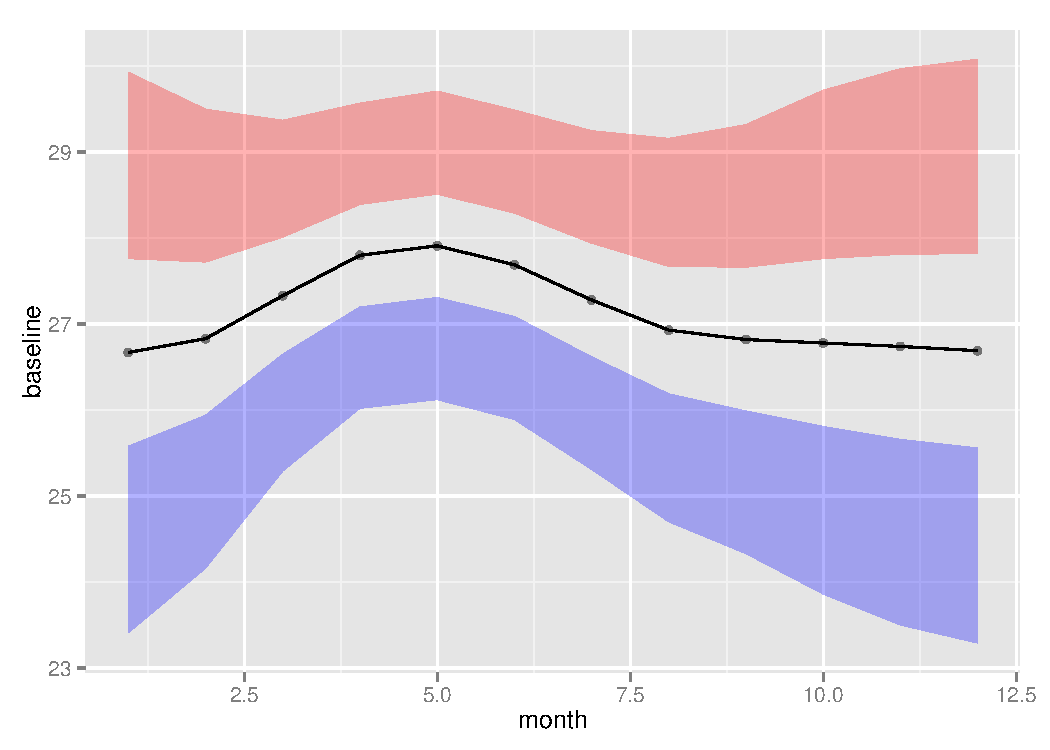
\includegraphics[width=\linewidth]{img/optionParamsByMonth.pdf}
  \caption{Index values for El \text{Ni\~no} (red) and La \text{Ni\~na} (blue) events between one and three standard deviations away from monthly average}
   \label{fig:optionParamsByMonth}
\end{figure}

Within those ranges, we use linear pricing such that an index value
halfway across the red band in figure \ref{fig:optionParamsByMonth}
(i.e.~halfway between the the trigger and max payout point) would
obligate a payout that is half of the max payout (sum insured, in
insurance terms) on a El \text{Ni\~no} contract. The full linear
function for October El \text{Ni\~no} is shown in figure
\ref{fig:payouyt10callex}.

Equation \ref{eq:calloption} represents the payout function for a long
call option spread on a monthly SST index. Long call option spreads pay
out to the hedger in circumstances where the underlying index increases,
hence they provide El \text{Ni\~no} protection, in this context. \(t\)
is the monthly temperature. For all the following examples we have
chosen October. \(a\) is the attachment point which in the following
examples is set at one standard deviation above the mean. For October
the attachment point for El \text{Ni\~no} protection is
\(27.76^{\circ}\mathrm{C}\). \(b\) is the exhaustion point, after which
payments do not increase. It is set at three standard deviations above
the mean in all El \text{Ni\~no} protection examples, or
\(29.72^{\circ}\mathrm{C}\) for October. (Note, that the attachment and
exhaustion points that define an options trade are collectively called
strikes.) This function is shown graphically in figure
\ref{fig:payouyt10callex}.

\begin{equation}
 F(t)=\left \{ \begin{array} {ll}
0 & \text{if} \,\, t \le a \\
\frac{t-a}{b-a} & \text{if} \,\, a<t<b\\
1 & \text{if} \,\, t \ge b\\
\end{array} \right.
\label{eq:calloption}
\end{equation}

\begin{figure}[!htbp]
  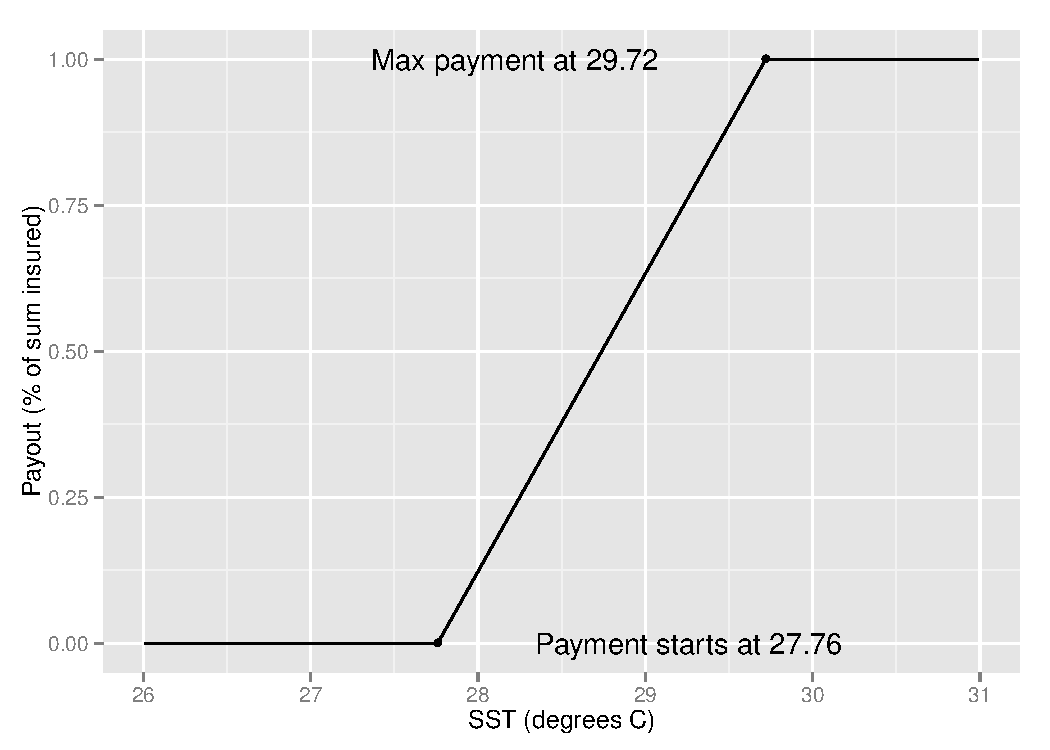
\includegraphics[width=\linewidth]{img/payoutExamplemonth10contractType1.pdf}
  \caption{Payout function for long call option spread (equivalent to El \text{Ni\~no} coverage) on October SST for \text{Ni\~no} 3.4 ERSST.3b trigged by index values between one and three standard deviations above the monthly baseline.}
   \label{fig:payouyt10callex}
\end{figure}

As an example, suppose that a Peruvian bank bought USD \(100\) of
coverage against October El \text{Ni\~no}. If actual October SST was
halfway across the red band, or \(28.74^{\circ}\mathrm{C}\), the bank
would receive USD \(50\). Figure \ref{fig:Compare1} shows the
obligations triggered by historic El \text{Ni\~no} events (measured in
October) if they were covered by this type of long call option spreads.
These loss estimates are equivalent to what is called in insurance a
\emph{burn rate}.

\begin{figure}[!htbp]
  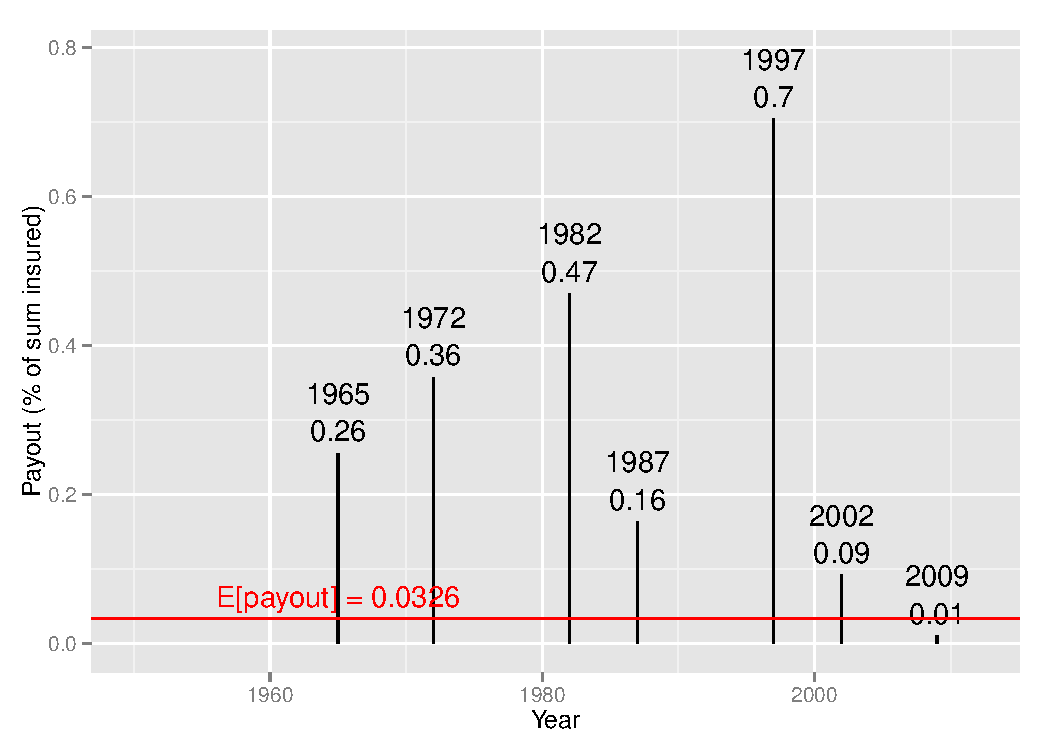
\includegraphics[width=\linewidth]{img/payoutBurnPlotmonth10contractType1.pdf}
  \caption{Historical burn on long call option spread for October SST for \text{Ni\~no} 3.4 ERSST.3b covering index values between one and three standard deviations above the baseline}
   \label{fig:Compare1}
\end{figure}

In practice, GlobalAgRisk found that hedgers (and speculators) prefer a
payout function that offers a minimum payout in the event that the index
reaches just above the trigger. For example, an index value that just
barely crosses into the red in figure \ref{fig:optionParamsByMonth}
might trigger a payout of \(5\) percent on an El \text{Ni\~no} contract,
rather than the tiny payout suggested the kind of linear function in
figure \ref{fig:payouyt10callex}.

\subsection{Distribution}\label{distribution}

Figure \ref{fig:optionPricesWithVariousDistMonth} provides month by
month expected prices El \text{Ni\~no} protection between one and three
standard deviations. (They are are unconditional on forecasts meaning
that they are equivalent to actuarially-fair insurance prices offered
prior to an insurance sales closing date.) They are denominated in USD
of premium per USD 100 of nominal coverage. The figure includes
historical burn prices, prices generates using non-parametric kernel
density smoother fit to historical data, as well as prices based on
various distributional fits (Jewson and Brix 2005).

\begin{figure}[!htbp]
  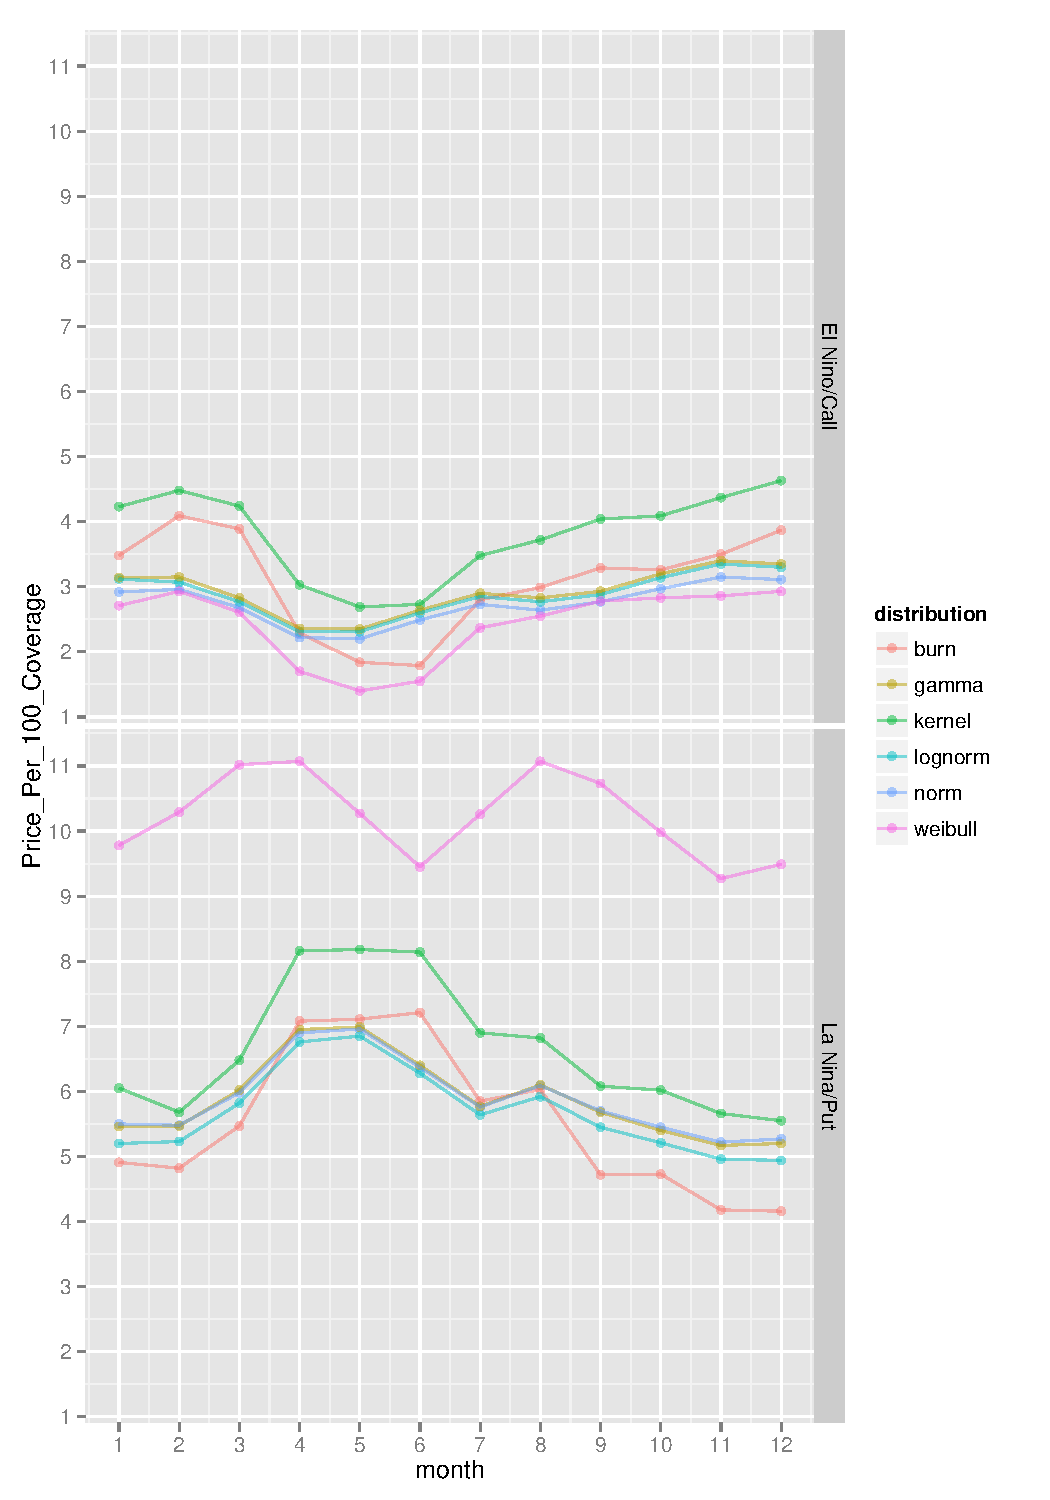
\includegraphics[width=\linewidth]{img/optionPricesWithVariousDistMonth.pdf}
  \caption{Expected price for options on \text{Ni\~no} 3.4 by month, based on simulations from various distributions}
   \label{fig:optionPricesWithVariousDistMonth}
\end{figure}

The prices in figure \ref{fig:optionPricesWithVariousDistMonth} appear,
with one prominent exception,\footnote{The prices from the Weibull
  samples are clearly distinct from the rest of the group - almost
  doubling the price of La \text{Ni\~na} coverage relative to the rest
  of the group. That is understandable given the distribution's heavy
  left tail. There is no indication that the process generating ENSO SST
  has a heavy left tail, so the distribution may not be appropriate
  here.} close to one another. However, they remain far enough apart
that hedgers would certainly notice a difference between the prices
offered by speculators insisting on the most conservative pricing
assumptions and those of speculators willing to offer coverage at prices
matching some weighted model average. On the El \text{Ni\~no} side, the
highest and lowest prices are generally within 125 basis points (1.25
percent) of one another in any given month. On the La \text{Ni\~na}
side, that spread is slightly larger at roughly 150 basis point, but
only between April and June.

Based on recent estimates of the risk premium on \emph{off-peak} risks
in catastrophe bond markets (those risks which are rarely managed in
catastrophe bond markets and thus are valued for their diversification
benefits), speculators demand a somewhere between 200 and 400 basis
points above expected loss (Ursano 2013). Using that benchmark, an
October option position covering El \text{Ni\~no} events between one and
three standard deviations from the monthly baseline priced using the
normal distribution might cost roughly 675 basis points. The same
position priced using a kernel density smoother might cost 800 basis
points, almost 20 percent higher.

The implied price difference illustrates two important points for
climate scientists looking to encourage the development of markets for
protection against the risks they study. First, distributional
assumptions have important economic consequences for risk markets
settling on direct climate indexes. In the case of ENSO, there is past
climate literature using a normal distribution to model ENSO. As we
discuss in the next section, we follow that precedence here while
allowing room for key modeling parameters to shift across a large search
space. However, further research on the appropriate distributions for
pricing climate risks will expedite the formation of stable, active risk
markets.

\section{Pricing ENSO risk contingent on available
forecasts}\label{pricing-enso-risk-contingent-on-available-forecasts}

Extreme El \text{Ni\~no}/La \text{Ni\~na} events emerge over time, with
forecasts giving us ever more reliable information in the months leading
up to a given event changing the beliefs of ENSO watchers.
Theoretically, a two-sided market in ENSO risk will quickly reflect
those changing beliefs and provide welfare enhancing forecast
information to the public through its prices. In practice, ENSO's
emerging risk profile could also create informational asymmetries that
undermine trading.

Publicly available pricing benchmarks would undermine such informational
asymmetries. With a strong pricing benchmark, such as an arbitrage
pricing formula, some highly specialize traders may still retain a
consistent edge over relatively naive traders, but the scope of that
edge is checked by public information. As long as it remains
sufficiently narrow, hedgers will remain in the market despite fears
that they are at an informational disadvantage.

This section provides such a benchmark. We present statistical
simulations of monthly \text{Ni\~no} 3.4 sea surface temperatures
conditioned on average forecasts released by Colombia University's
International Research Institute for Climate and Society (IRI). We use
those simulations to update the prices of risk management contracts as
new forecast information becomes available.

\subsection{Forecasts of ENSO SSTs}\label{forecasts-of-enso-ssts}

Before discussing the statistical treatment of forecasts, it is worth
quickly reviewing the ENSO SST forecasts provided by IRI because those
forecasts are offered in a format that is not directly comparable to the
format we believe is most appropriate for traded \text{Ni\~no} risk
protection.

Every month since mid-2002, IRI has collected forecasts issued by major
centers of climatological research. Figure \ref{fig:forecastExamples}
shows IRI the forecasts as of March 2013.

\begin{figure}
  \begin{center}
  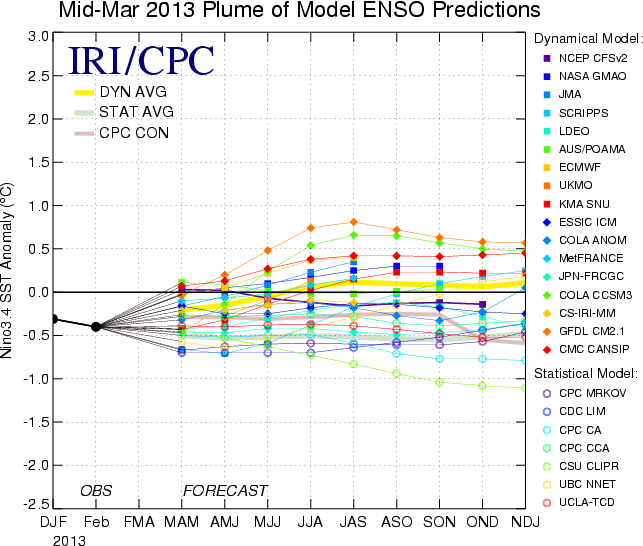
\includegraphics[width=.5\linewidth]{img/SST_table_march_ex.png}
  \caption{Example of IRI's collected forecasts - March 2013}
   \label{fig:forecastExamples}
   \end{center}
\end{figure}

IRI provides \text{Ni\~no} 3.4 anomaly SST forecasts over three month
rolling windows. As discussed previously, monthly SSTs are likely better
suited to risk trading. To provide an index of IRI forecasts that is
directly comparable to the monthly SSTs that we wish to price, we have
averaged all the available IRI forecasts that cover a given month. For
an example of how we made this simplification, imagine that it is March
and a hedger is interested in predicting October \text{Ni\~no} 3.4 SST.
In figure \ref{fig:forecastExamples}, there are three forecasts that
contain information relevant to October SSTs - \emph{ASO}, \emph{SON},
and \emph{OND}. In that case our forecast index is the average of those
three numbers.

IRI issues forecasts between 2 and 10 months prior to any given target
month. For example, October SST forecasts begin in December and end in
September.

\subsection{Linking forecasts to outcomes ENSO
SSTs}\label{linking-forecasts-to-outcomes-enso-ssts}

We generate stochastic catalogs of ENSO outcomes conditional on the IRI
average forecasts discussed above using the Bayesian regression in
equation \ref{eqn:conditionalEstEqn}. This a simplified version of a
procedure that climate scientists and statisticians have recently used
to merge ENSO forecasts (Luo, Wood, and Pan 2007; Coelho et al. 2004).
Since we want pricing for every month, from the vantage-point of every
preceding month with IRI forecasts (nine forecasts, starting ten months
prior to the target month), we run a total of \(108\) separate
regressions.

Note first that we do not know the predictive power of IRI average
forecasts a priori. The parameter \(\sigma_{y_{to,from}}^2\) accounts
for that forecasting uncertainty. It will be large where IRI average
forecasts have shown low historical predictive power. Note also that
this Bayesian regression will not be biased by non-stationarity. The
underlying parameters are not assumed to be stationary, since they are
realizations of an unknown distribution.

\begin{equation}
\begin{array}{lcl}
\mbox{Monthly Ni\~no 3.4 ERSST.3b anomalies}_{to,year} & \sim & \mathcal{N}( \hat{y}_{to,from,year}, \sigma_{y_{to,from}}^2 )\\
\hat{y}_{to,from,year} & = & a_{to,from}+\\
&& b_{to,from}*\\
&& \mbox{IRI average}_{to,from}\\
\end{array}
\label{eqn:conditionalEstEqn}
\end{equation}

The prior probabilities placed on model parameters are shown in equation
set \ref{eqn:priorsconditionalEstEqn}. \(to\) represents the month
targeted by the forcast, \(from\), the month in which the forecast is
made, and \(year\), the year of the SST measurement. There are weakly
informative priors on \(b\) and \(\sigma_{y}\), allowing them to move
easily across a wide range of possible values in response to the data.
\(a\) by contrast has a strongly informative prior based on historical
data. This means that if \(b\), the parameter indicating the predictive
power of IRI's average forecasts, is at or near zero, then the resulting
simulations from the posterior distribution will simply reflect long
term trends in monthly SSTs.

\begin{equation}
\begin{array}{lcl}
a_{to,from}  & \sim & \mathcal{N}(\mbox{mean anomalies}_{to}, \mbox{st dev anomalies}_{to}) \\
b_{to,from}  & \sim & \mathcal{N}(0, 100) \\
\sigma_{y_{to,from}}^2 & \sim  &\mbox{Inv gamma}(0.001, 0.001) \\
\end{array}
\label{eqn:priorsconditionalEstEqn}
\end{equation}

\subsubsection{Dynamic pricing based on model
results}\label{dynamic-pricing-based-on-model-results}

The table below contains regression results for October SSTs, predicted
between the preceding December and August. The regressions were all
estimated using the Bayesian estimation program STAN with four parallel
Markov Chain Monte Carlo (MCMC) chains, each with 100,000 iterations,
50,000 of which were discarded as a warm-up (Stan Development Team
2013). The convergence statistic, \(\hat{R}\), on all parameters was
close to 1, indicating that the parallel MCMC chains showed convergent
results by the end of the simulation.

\begin{table}[!htbp]
\centering
\footnotesize
\begin{tabular}{rrrrrrrrrr}
\hline
\multicolumn{10}{c}{August forecast average covering October \text{Ni\~no} 3.4 SST anomalies}\\
  \hline
 & mean & sd & $2.5^{\mbox{th}}$ q & $25^{\mbox{th}}$ q & $50^{\mbox{th}}$ q & $75^{\mbox{th}}$ q & $97.5^{\mbox{th}}$ q & n\_eff & Rhat \\ 
  \hline
$\alpha$ & -0.10 & 0.10 & -0.40 & -0.20 & -0.10 & -0.10 & 0.10 & 91045 &   1 \\ 
  $\beta$ & 1.10 & 0.20 & 0.80 & 1.00 & 1.10 & 1.20 & 1.50 & 88920 &   1 \\ 
  $\sigma^{2}_{y}$ & 0.10 & 0.10 & 0.10 & 0.10 & 0.10 & 0.20 & 0.40 & 56829 &   1 \\ 
   \hline
\hline
\multicolumn{10}{c}{July forecast average covering October \text{Ni\~no} 3.4 SST anomalies}\\
  \hline
$\alpha$ & -0.10 & 0.20 & -0.50 & -0.20 & -0.10 & 0.00 & 0.20 & 92218 &   1 \\ 
  $\beta$ & 1.20 & 0.30 & 0.60 & 1.00 & 1.20 & 1.30 & 1.70 & 93712 &   1 \\ 
  $\sigma^{2}_{y}$ & 0.30 & 0.20 & 0.10 & 0.20 & 0.30 & 0.40 & 0.90 & 54297 &   1 \\ 
   \hline
\hline
\multicolumn{10}{c}{June forecast average covering October \text{Ni\~no} 3.4 SST anomalies}\\
  \hline
$\alpha$ & -0.10 & 0.20 & -0.40 & -0.20 & -0.10 & 0.00 & 0.30 & 95908 &   1 \\ 
  $\beta$ & 1.40 & 0.30 & 0.70 & 1.20 & 1.40 & 1.60 & 2.10 & 91107 &   1 \\ 
  $\sigma^{2}_{y}$ & 0.30 & 0.20 & 0.10 & 0.20 & 0.30 & 0.40 & 0.90 & 55596 &   1 \\ 
   \hline
\hline
\multicolumn{10}{c}{May forecast average covering October \text{Ni\~no} 3.4 SST anomalies}\\
  \hline
$\alpha$ & -0.10 & 0.20 & -0.50 & -0.20 & -0.10 & 0.10 & 0.40 & 92919 &   1 \\ 
  $\beta$ & 1.50 & 0.60 & 0.40 & 1.20 & 1.50 & 1.90 & 2.60 & 90255 &   1 \\ 
  $\sigma^{2}_{y}$ & 0.50 & 0.30 & 0.20 & 0.30 & 0.50 & 0.60 & 1.40 & 59205 &   1 \\ 
   \hline
\hline
\multicolumn{10}{c}{April forecast average covering October \text{Ni\~no} 3.4 SST anomalies}\\
  \hline
$\alpha$ & -0.10 & 0.20 & -0.50 & -0.30 & -0.10 & 0.00 & 0.30 & 88326 &   1 \\ 
  $\beta$ & 1.90 & 0.60 & 0.70 & 1.50 & 1.90 & 2.30 & 3.00 & 83902 &   1 \\ 
  $\sigma^{2}_{y}$ & 0.40 & 0.30 & 0.20 & 0.30 & 0.40 & 0.50 & 1.10 & 57674 &   1 \\ 
   \hline
\hline
\multicolumn{10}{c}{March forecast average covering October \text{Ni\~no} 3.4 SST anomalies}\\
  \hline
$\alpha$ & 0.00 & 0.20 & -0.50 & -0.10 & 0.00 & 0.20 & 0.50 & 101040 &   1 \\ 
  $\beta$ & 1.80 & 0.90 & 0.00 & 1.20 & 1.80 & 2.30 & 3.50 & 96782 &   1 \\ 
  $\sigma^{2}_{y}$ & 0.70 & 0.50 & 0.30 & 0.50 & 0.60 & 0.90 & 1.90 & 59539 &   1 \\ 
   \hline
\hline
\multicolumn{10}{c}{February forecast average covering October \text{Ni\~no} 3.4 SST anomalies}\\
  \hline
$\alpha$ & -0.10 & 0.30 & -0.70 & -0.30 & -0.10 & 0.10 & 0.60 & 98192 &   1 \\ 
  $\beta$ & 0.80 & 1.30 & -1.80 & 0.00 & 0.80 & 1.60 & 3.40 & 88684 &   1 \\ 
  $\sigma^{2}_{y}$ & 1.10 & 0.80 & 0.40 & 0.60 & 0.90 & 1.30 & 3.20 & 54912 &   1 \\ 
   \hline
\hline
\multicolumn{10}{c}{January forecast average covering October \text{Ni\~no} 3.4 SST anomalies}\\
  \hline
$\alpha$ & 0.00 & 0.30 & -0.60 & -0.20 & 0.00 & 0.20 & 0.60 & 99518 &   1 \\ 
  $\beta$ & 1.00 & 1.60 & -2.30 & 0.00 & 1.00 & 2.00 & 4.20 & 92225 &   1 \\ 
  $\sigma^{2}_{y}$ & 1.00 & 0.70 & 0.40 & 0.60 & 0.80 & 1.20 & 2.80 & 55715 &   1 \\ 
   \hline
\hline
\multicolumn{10}{c}{December forecast average covering October \text{Ni\~no} 3.4 SST anomalies}\\
  \hline
$\alpha$ & 0.00 & 0.30 & -0.60 & -0.20 & 0.00 & 0.30 & 0.70 & 80946 &   1 \\ 
  $\beta$ & -0.30 & 1.90 & -4.00 & -1.40 & -0.30 & 0.90 & 3.50 & 76663 &   1 \\ 
  $\sigma^{2}_{y}$ & 1.10 & 0.70 & 0.40 & 0.60 & 0.90 & 1.30 & 2.90 & 56323 &   1 \\ 
   \hline
\end{tabular}
\caption[Bayesian regression linking October \text{Ni\~no} 3.4 SST anomalies to average of relevant IRI ensemble forecasts]{Bayesian regression linking October \text{Ni\~no} 3.4 SST anomalies to average of relevant IRI ensemble forecasts} 
\label{tab:regOfConditionalsTablemonth10}
\end{table}

Looking at the 2.5th and 97.5th percentile of the distributions for
\(b\), its clear that the forecasts become more valuable as the year
goes on. Going from December to August, the 95 percent probability
interval for the forecast parameter, \(b\) steadily tightens to a range
including 1. This suggest that the correlation between forecasts and
eventual SSTs increases throughout the predictive window. As the
explanatory value of \(b\) increases, \(a\) decreases. \(a\)'s 95
percent probability tightens around 0 after March indicating that there
are no consistent patterns of IRI forecasts being too high or too low
relative to observed SSTs after March.

Using the posterior draws of parameter values from these 108
regressions, we simulated SSTs predicted by each possible forecast value
between -2 and 2 (forecasts are rounded to one decimal). For example, we
took 50,000 posterior draws of \(a\), \(b\), and \(\sigma_{y}^2\) from
the regression corresponding to October SSTs predicted by April
forecasts. Each of those 50,000 vectors of three parameters were used to
randomly generate one October SST based on an average April forecast of
mild El \text{Ni\~no} conditions in the coming October (a forecast value
of 0.5). That gave a stochastic catalog of 50,000 October SSTs
conditioned on a forecast of 0.5 made in April. We repeated that
procedure to produce conditional distributions for SSTs for each month
of the year, predicted by a wide range of forecast values, from all
possible forecast months.

The empirical cumulative distribution functions (ECDFs) of those
posterior simulations, converted back into absolute SSTs,\footnote{We
  have also touched on why the choice between anomalies and absolute
  SSTs is of lower importance than some of the other choices facing the
  launch of traded ENSO markets. Our statistical routines linking
  forecasts to outcomes are in terms of anomalies. However, financial
  professionals unfamiliar with ENSO SST indexes may benefit from seeing
  the absolute temperates because they show the natural fluctuations in
  Pacific SSTs throughout the year which have been taken out of anomaly
  figures. In recognition of that fact, the conditional cumulative
  distribution functions below are in terms of absolute degrees.} are
shown in figures \ref{fig:conditionalCDFs04to06},
\ref{fig:conditionalCDFs07to09}, \ref{fig:conditionalCDFs10to12}, and
\ref{fig:conditionalCDFs01to03}.

\begin{figure}[!htbp]
  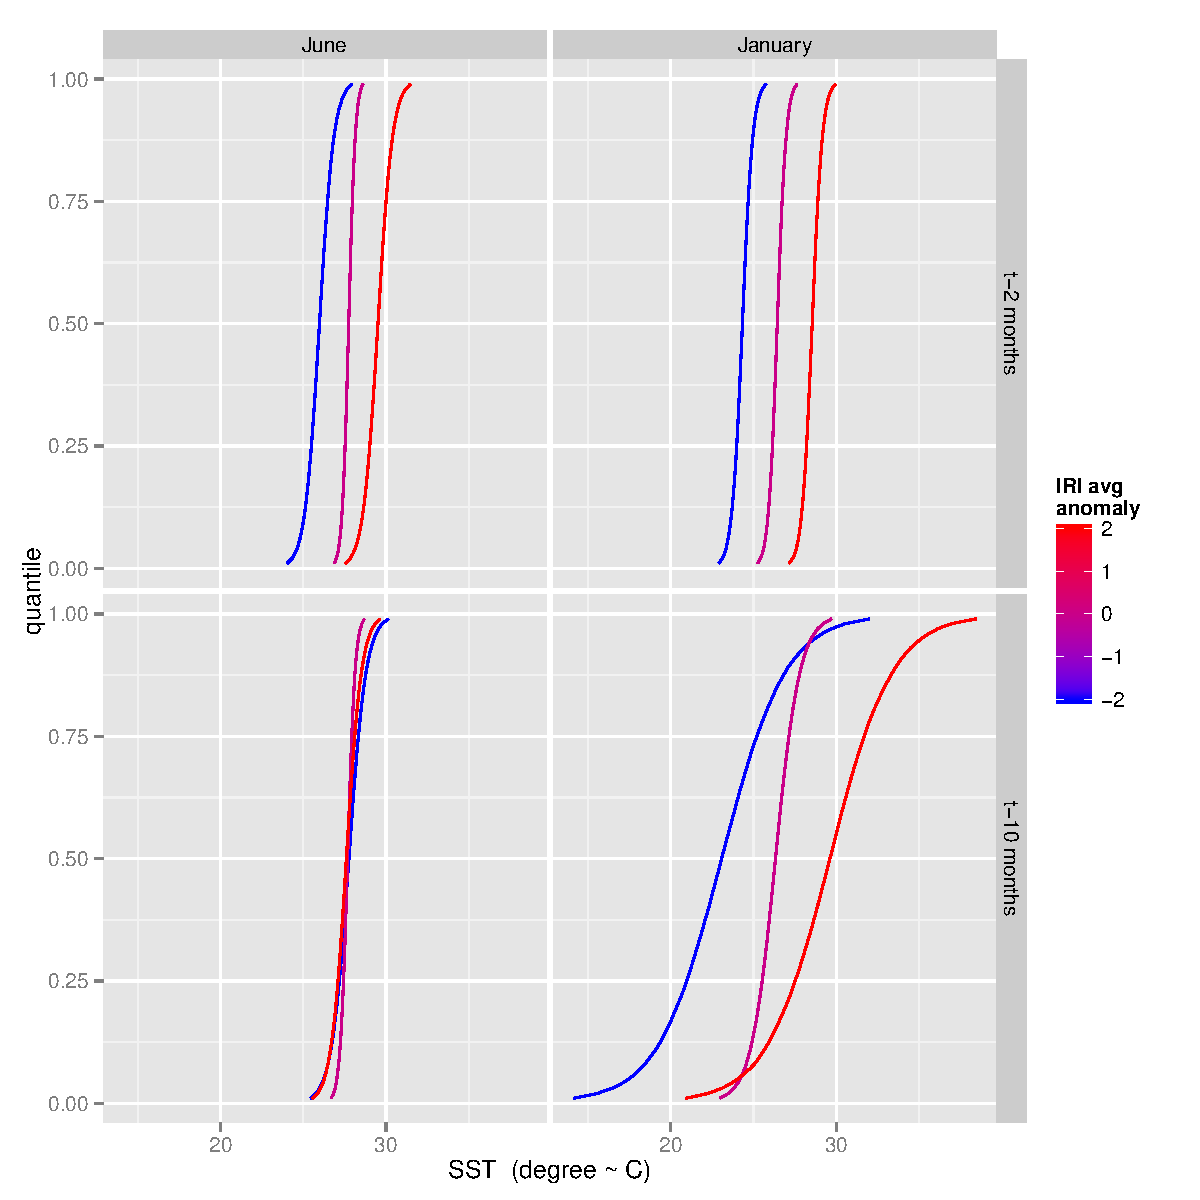
\includegraphics[width=\linewidth]{img/conditionalCDFsIllustrativeExamplesTradConfigSimple.pdf}
  \caption{Empirical cumulative distribution functions for June and January \text{Ni\~no} 3.4 SST conditioned on average IRI ensemble forecasts available for various months. Only the ECDFs for the nearest and furthest month predictions provided by IRI and only predictions of large El \text{Ni\~no} (+2), La \text{Ni\~na} (-2), or neutral conditions (0) are shown. ECDFs are of draws from the posterior predictive distribution of the model specified in equation \ref{eqn:conditionalEstEqn}.}
   \label{fig:conditionalCDFsIllustrativeExamplesTradConfigSimple}
\end{figure}

Figure \ref{fig:conditionalCDFsIllustrativeExamplesTradConfigSimple}
presents a highly simplified example of these ECDFs. It has just two
target months (June and January), two windows from which predictions of
SSTs in those target month were made (two and ten months prior to the
target month) and three prediction values (a +2 anomaly suggesting
strong El \text{Ni\~no}, indicated by the deepest red line, a -2 anomaly
suggesting strong La \text{Ni\~na}, indicated by the deepest blue line,
and no anomaly suggesting neutral conditions, indicated by the purple
line). The highest simulated SSTs conditioned on a given forecast at
then upper right-hand end of each line, with the simulation result value
on the x-axis and the quantile of that result on the y-axis.

The pattern of these ECDFs tell a great deal about the predictive power
of IRI average forecasts and the underlying process of SSTs in a given
month. Note first that June is not a month with highly variable SSTs.
The purple line indicating the ECDF conditioned on neutral forecasts is
almost vertical, both when those forecasts are made in April and in
August of the preceding year. January SSTs show greater underlying
variability, with their ECDFs stretching further along the x-axis.

The longest dated forecasts (t-10 months) are not reliable for June but
show some value for January. This is shown by the overlap of the various
ECDFs. In June, they are stacked on top of one another, showing that
conditioning on forecasts produces roughly equivalent distributions of
outcomes. By contrast, extreme forecasts of El \text{Ni\~no} or La
\text{Ni\~na} were associated with January SSTs that were
distributionally distinct from one another (there is little overlap
between the lower tail of the red line and the upper tail of the blue
line) the with high confidence, even for forecasts made in March.
However, while a March forecast of El \text{Ni\~no} conditions in
January meant that we were unlikely to see extreme La \text{Ni\~na}
conditions, it did not rule out the range of outcomes associated with
neutral forecasts.

By the time that we are only two months away from our target months
however, extreme high and low forecasts are associated with a range of
outcomes that are distinct both from one another and from neutral
forecasts. This shows how the informational value of forecasts increases
as the forecast horizon gets shorter.

In figure \ref{fig:conditionalCDFsIllustrativeExamplesTradConfigFull}
the full complement of forecasts is shown for the same targets and
forecast horizons. Boxes where the red lines are consistently above the
blue lines indicate high informational value for forecasts, with a clear
distinction between outcomes associated with high and low forecasts.

\begin{figure}[!htbp]
  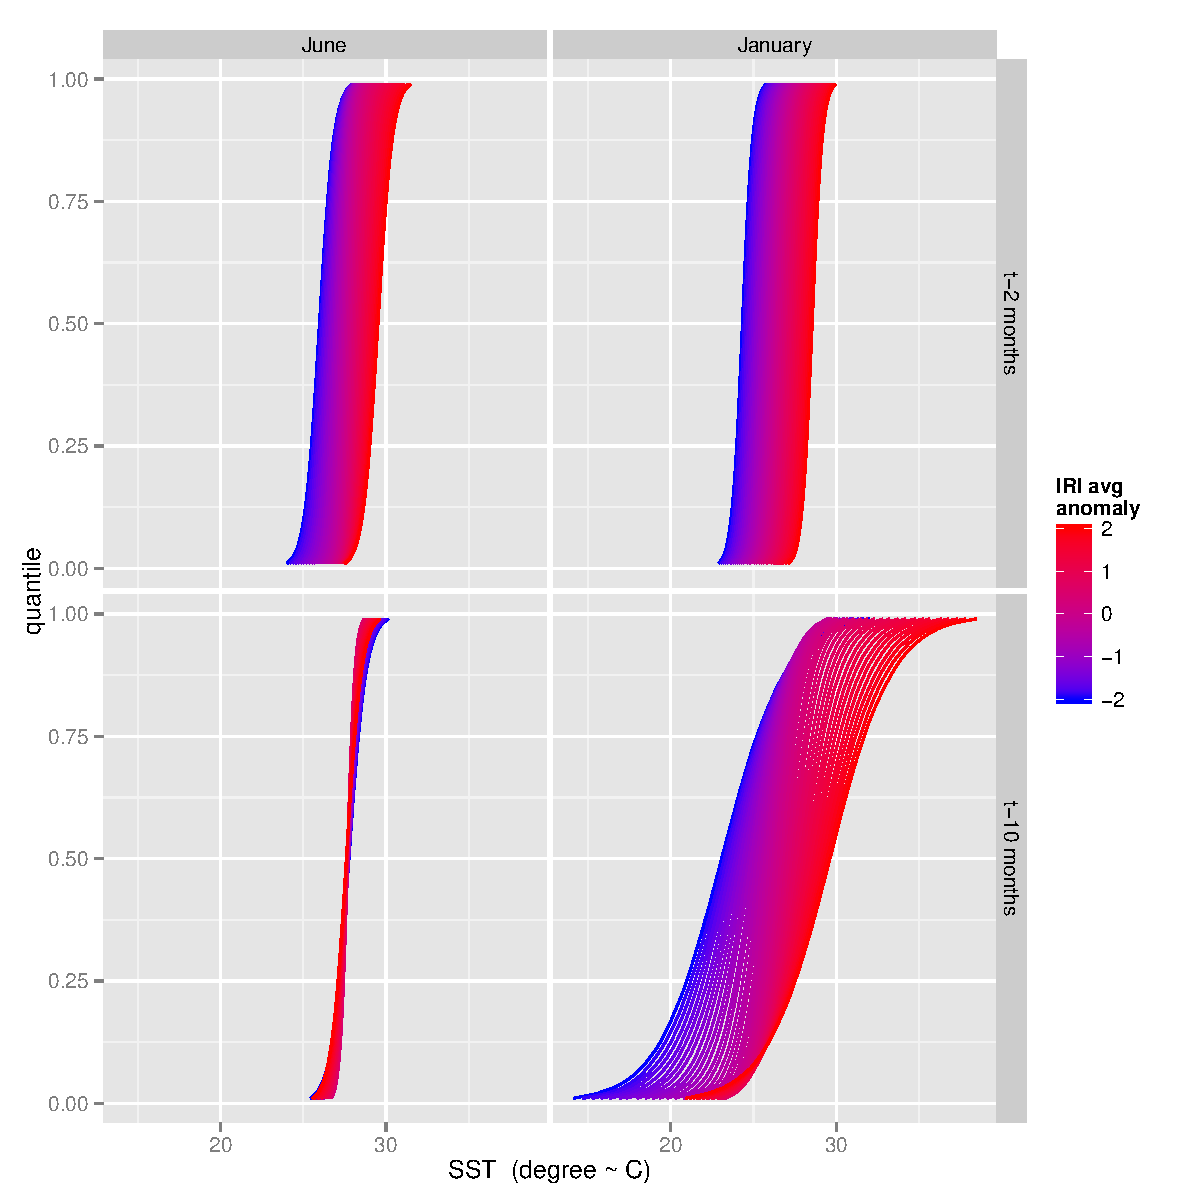
\includegraphics[width=\linewidth]{img/conditionalCDFsIllustrativeExamplesTradConfigFull.pdf}
  \caption{Empirical cumulative distribution functions for June and January \text{Ni\~no} 3.4 SST conditioned on average IRI ensemble forecasts available for various months. Only the ECDFs for the nearest and furthest month predictions provided by IRI are shown. ECDFs are of draws from the posterior predictive distribution of the model specified in equation \ref{eqn:conditionalEstEqn}.}
   \label{fig:conditionalCDFsIllustrativeExamplesTradConfigFull}
\end{figure}

With that simplified example in mind you can interpret patterns in the
full simulation results shown in figures
\ref{fig:conditionalCDFs04to06}, \ref{fig:conditionalCDFs07to09},
\ref{fig:conditionalCDFs10to12}, and \ref{fig:conditionalCDFs01to03}.
The blue and red lines are tightly bound ten months prior to any given
target month and in many cases the blue lines reach further right than
the red. This indicates that forecasts had little or no predictive
power. Warm forecasts were as closely associated with eventual warm
conditions as cold forecasts, and visa versa.

By contrast, two months away from a target month (the upper row of
figures \ref{fig:conditionalCDFs04to06},
\ref{fig:conditionalCDFs07to09}, \ref{fig:conditionalCDFs10to12}, and
\ref{fig:conditionalCDFs01to03}), forecasts are meaningful. Blue lines
sit below red lines. So a warm forecast shifts the distribution of
eventual SSTs warmer and visa versa.

\begin{figure}[!htbp]
\begin{center}
  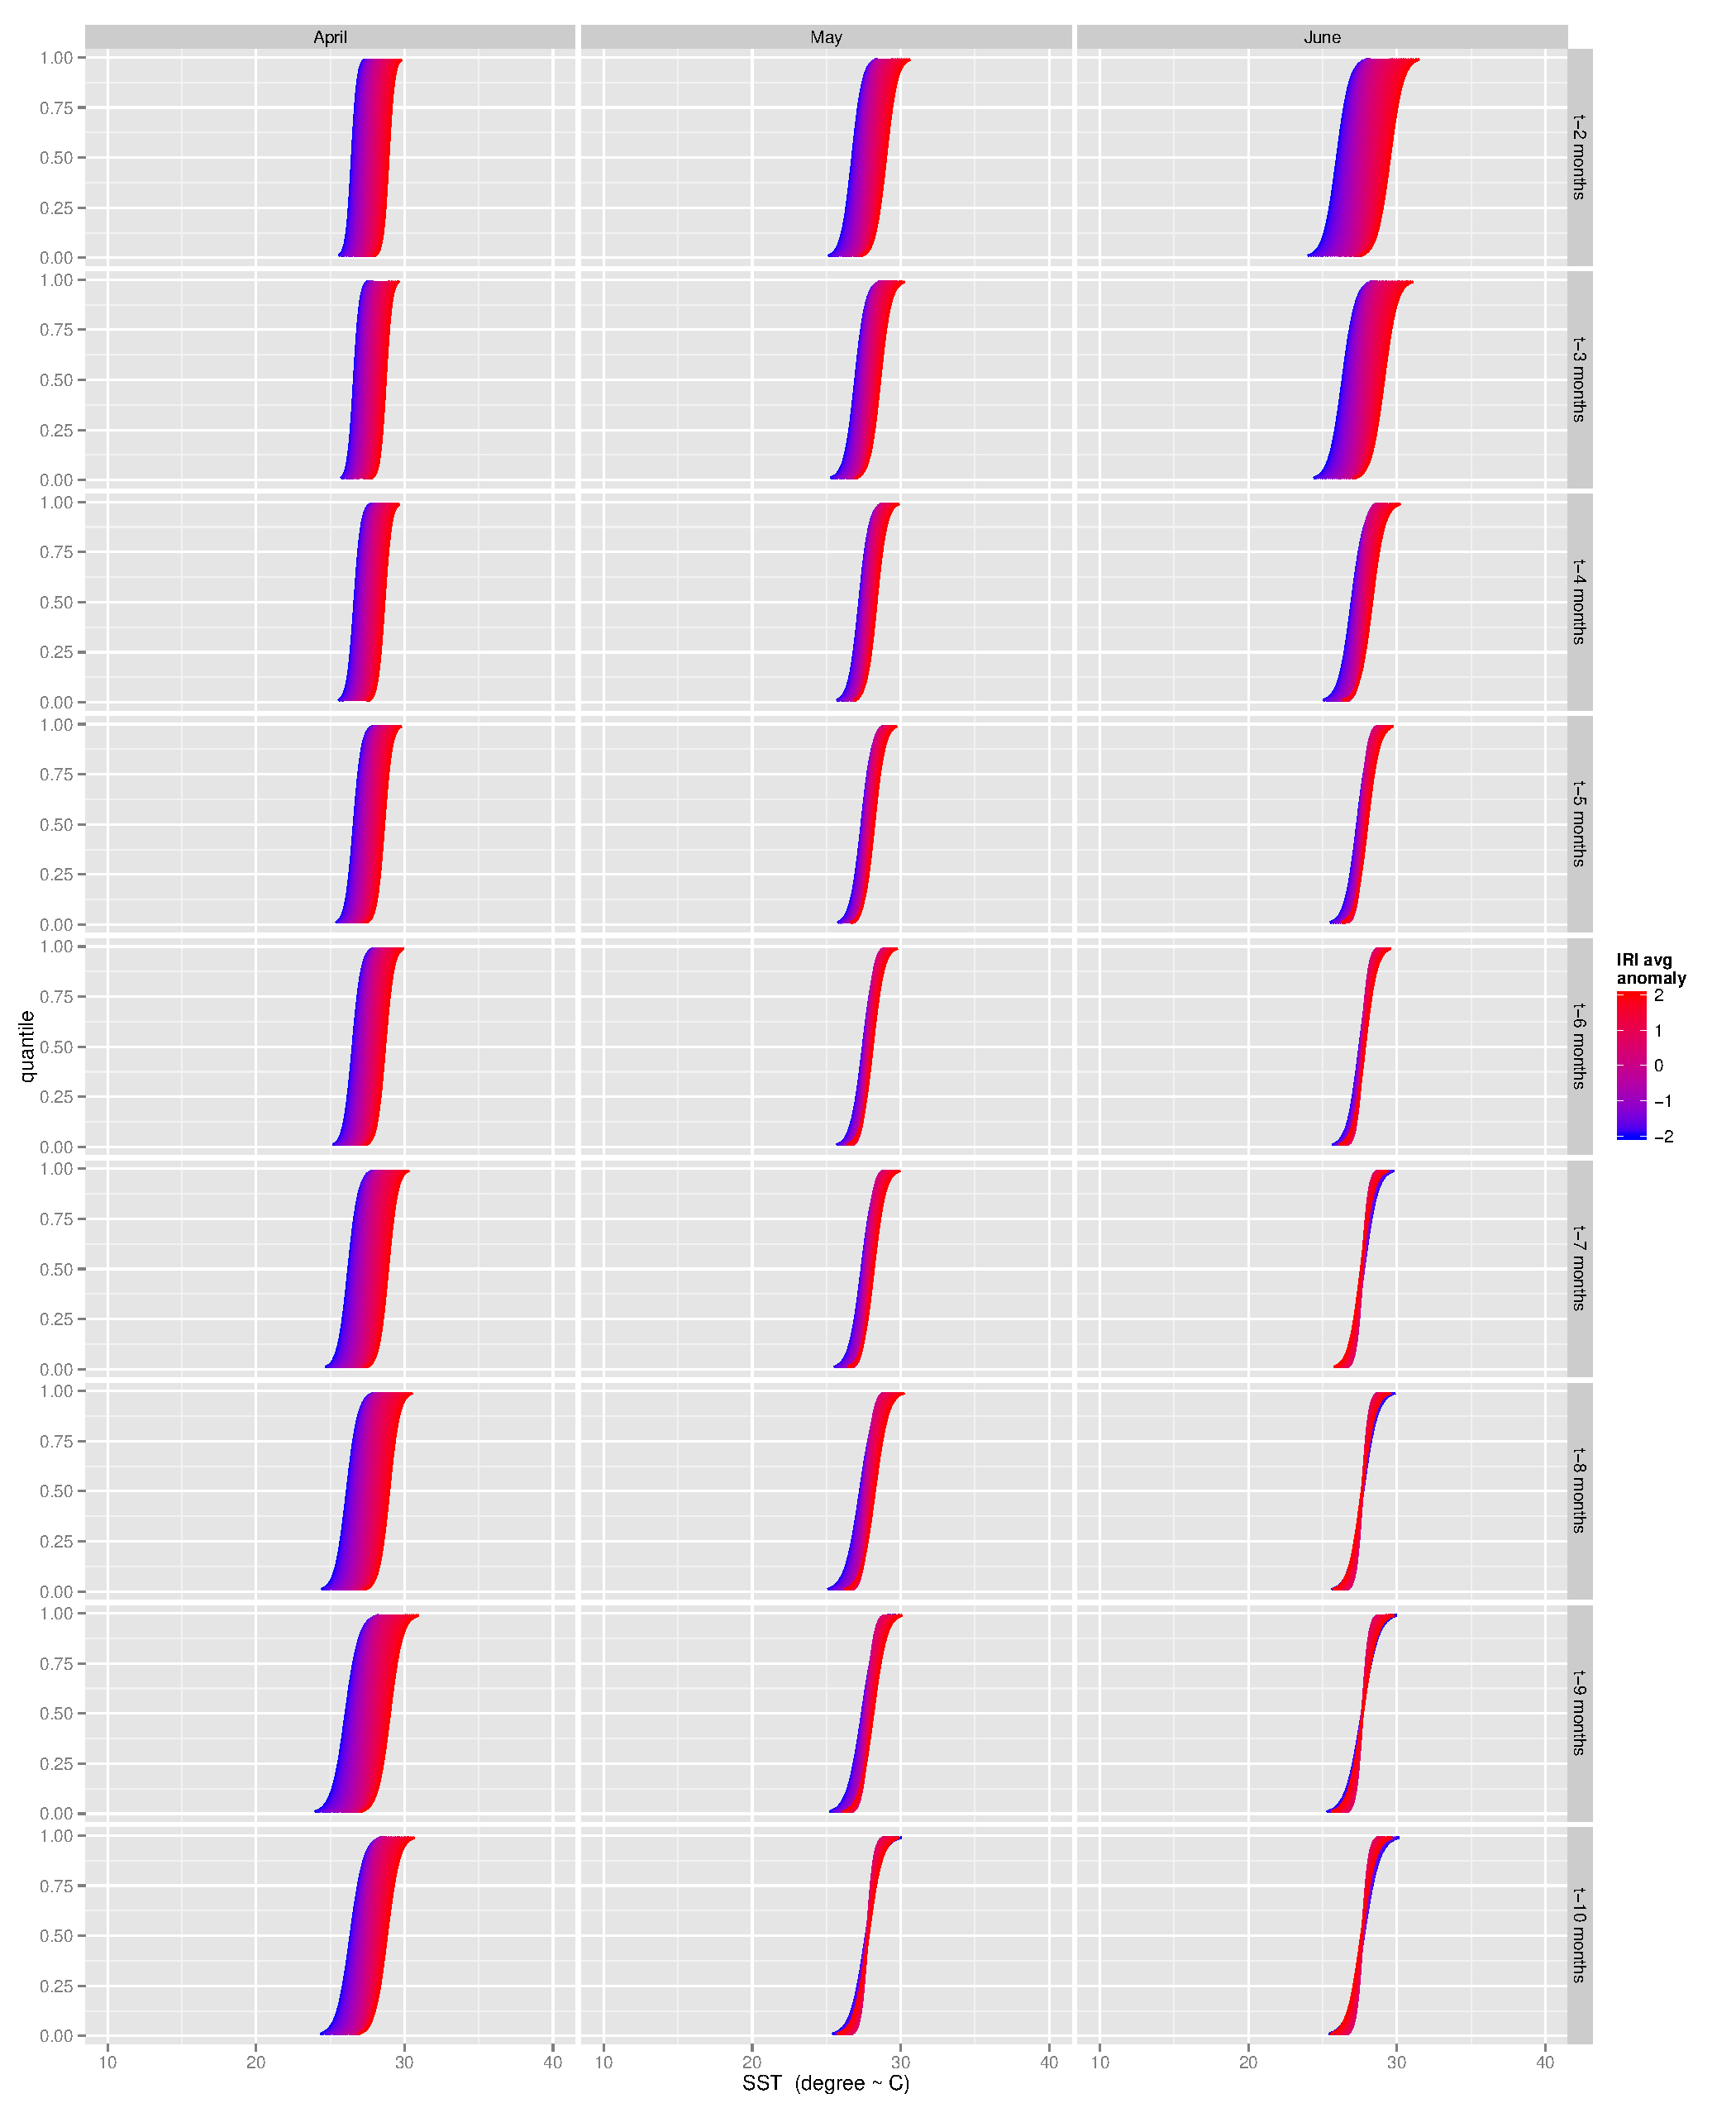
\includegraphics[width=\linewidth, keepaspectratio]{img/conditionalCDFs04to06TraditionalCDFconfig.pdf}
  \caption{Empirical cumulative distribution functions for April through June \text{Ni\~no} 3.4 SST conditioned on average IRI ensemble forecasts available for various months. ECDFs are of draws from the posterior predictive distribution of the model specified in equation \ref{eqn:conditionalEstEqn}.}
   \label{fig:conditionalCDFs04to06}
   \end{center}
\end{figure}

\begin{figure}[!htbp]
  \begin{center}
    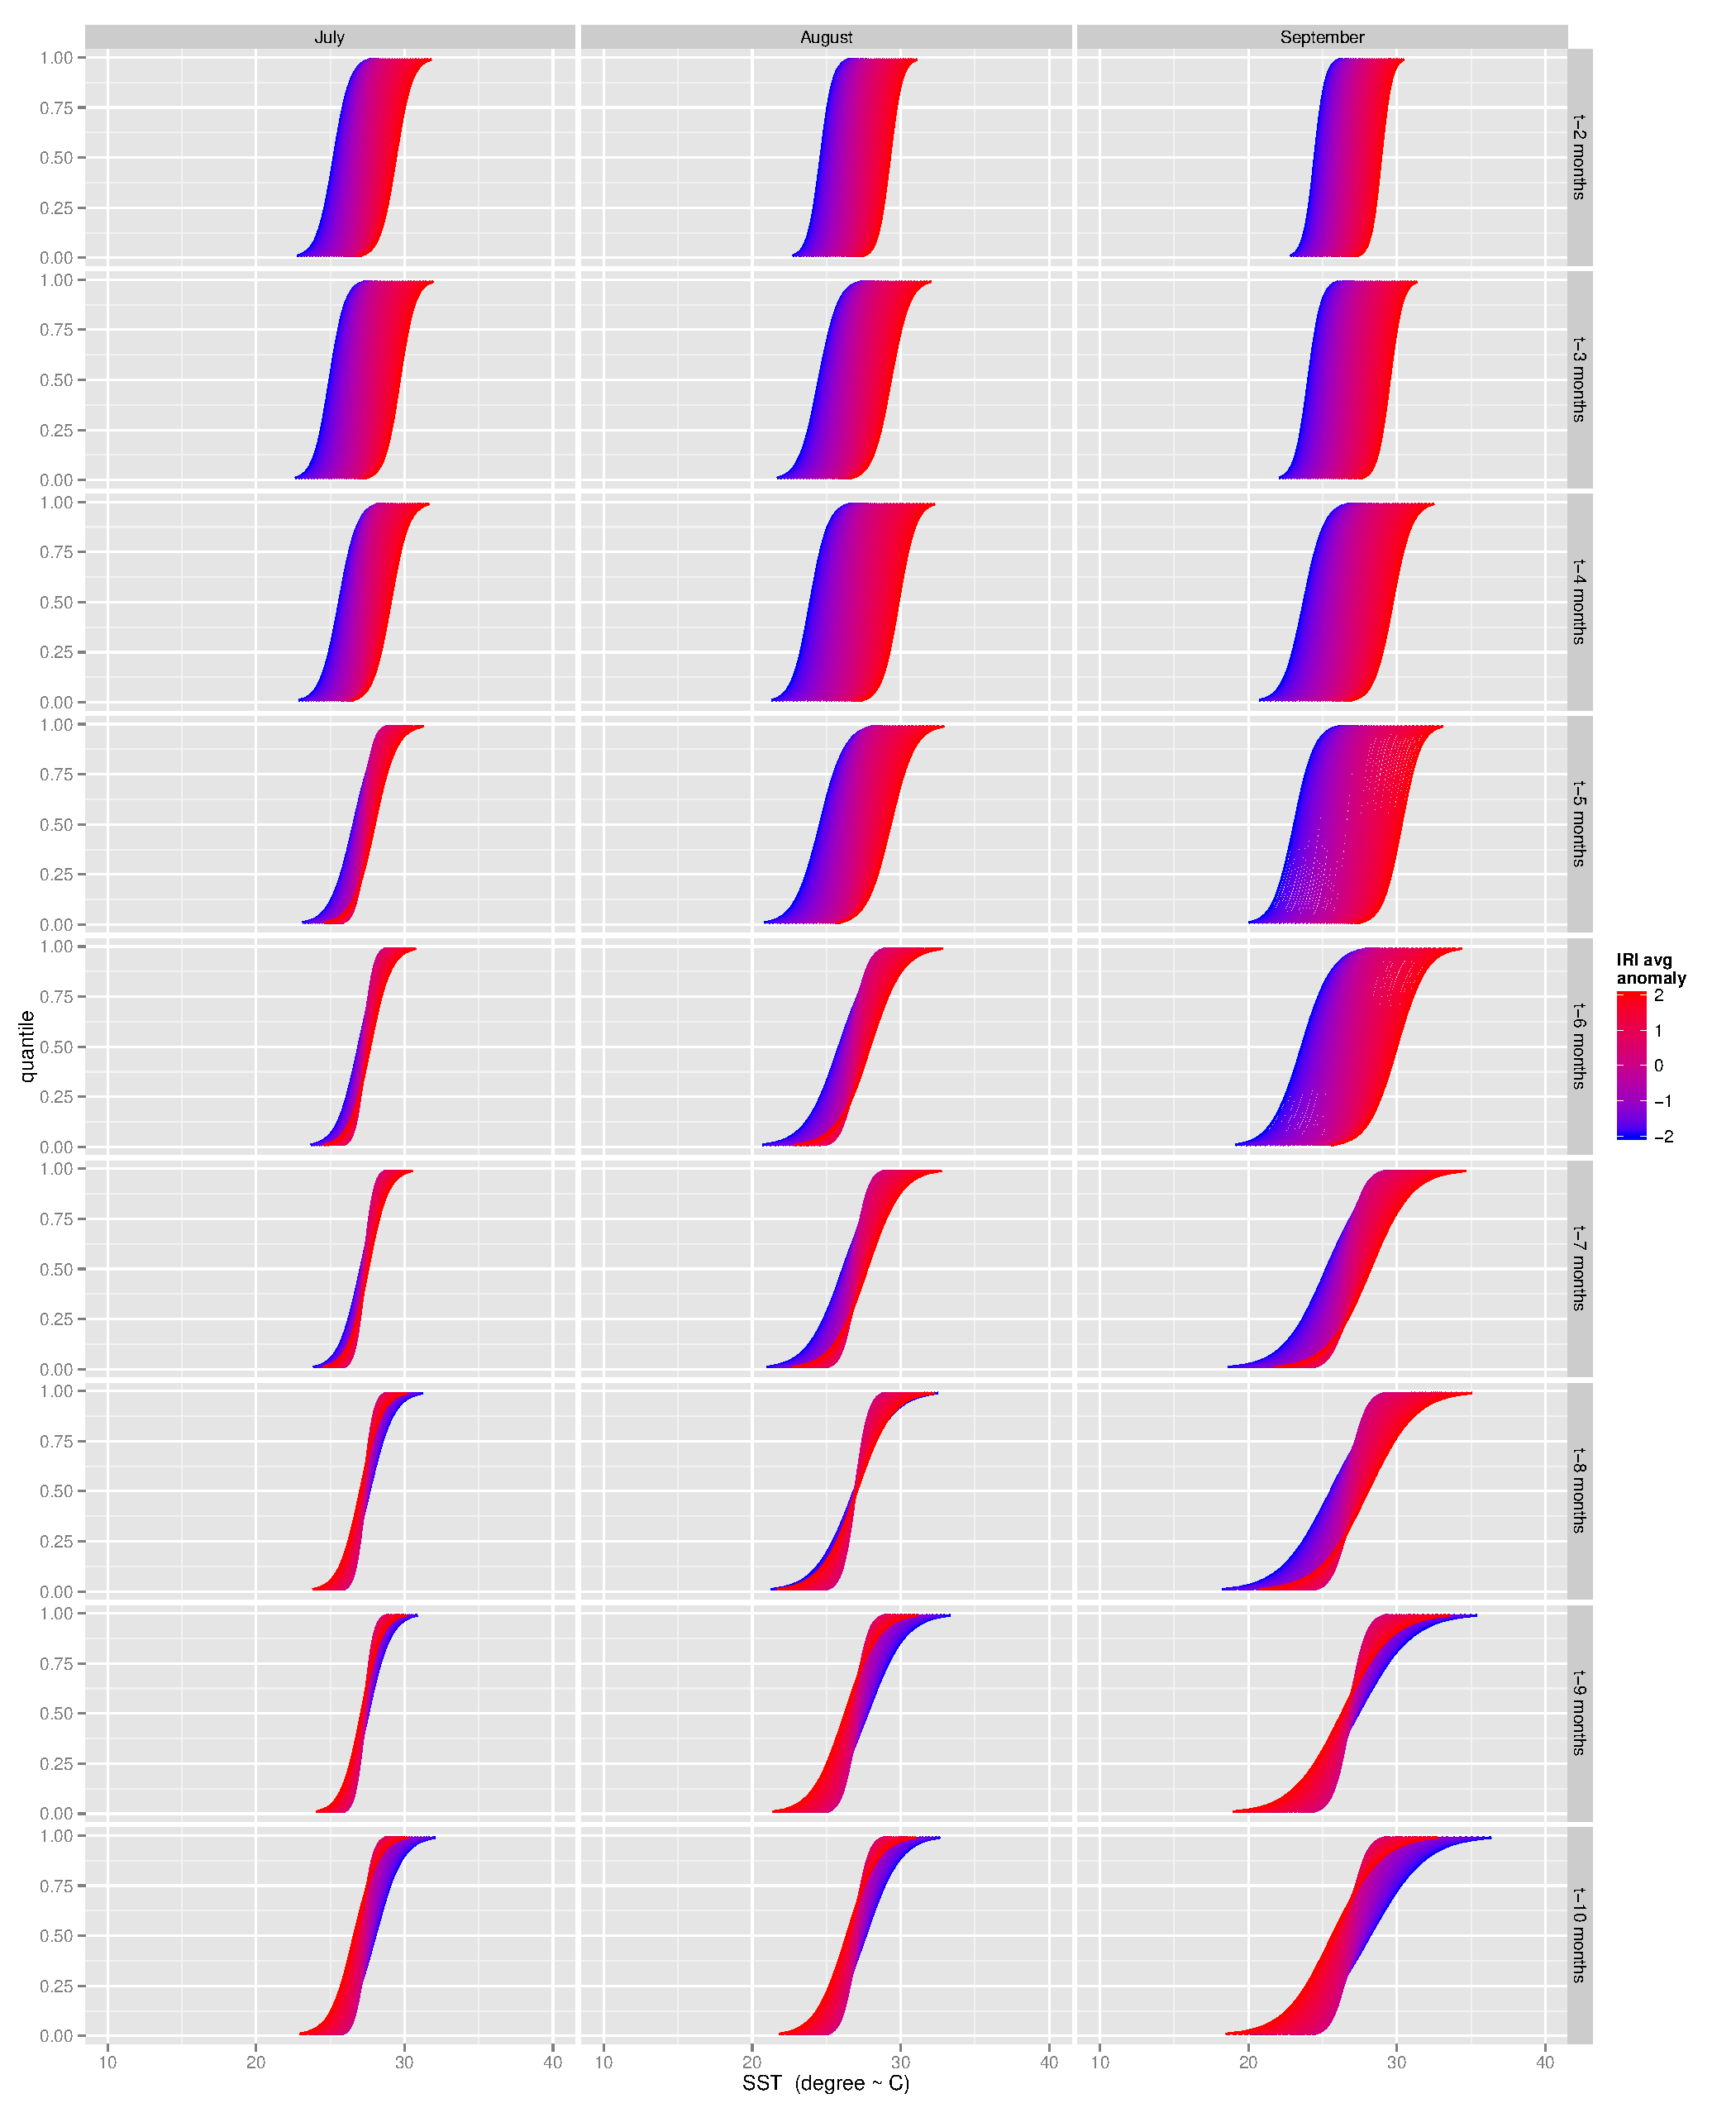
\includegraphics[width=\linewidth, keepaspectratio]{img/conditionalCDFs07to09TraditionalCDFconfig.pdf}
    \caption{Empirical cumulative distribution functions for July through September \text{Ni\~no} 3.4 SST conditioned on average IRI ensemble forecasts available for various months. ECDFs are of draws from the posterior predictive distribution of the model specified in equation \ref{eqn:conditionalEstEqn}.}
    \label{fig:conditionalCDFs07to09}
   \end{center}
\end{figure}

\begin{figure}[!htbp]
  \begin{center}
    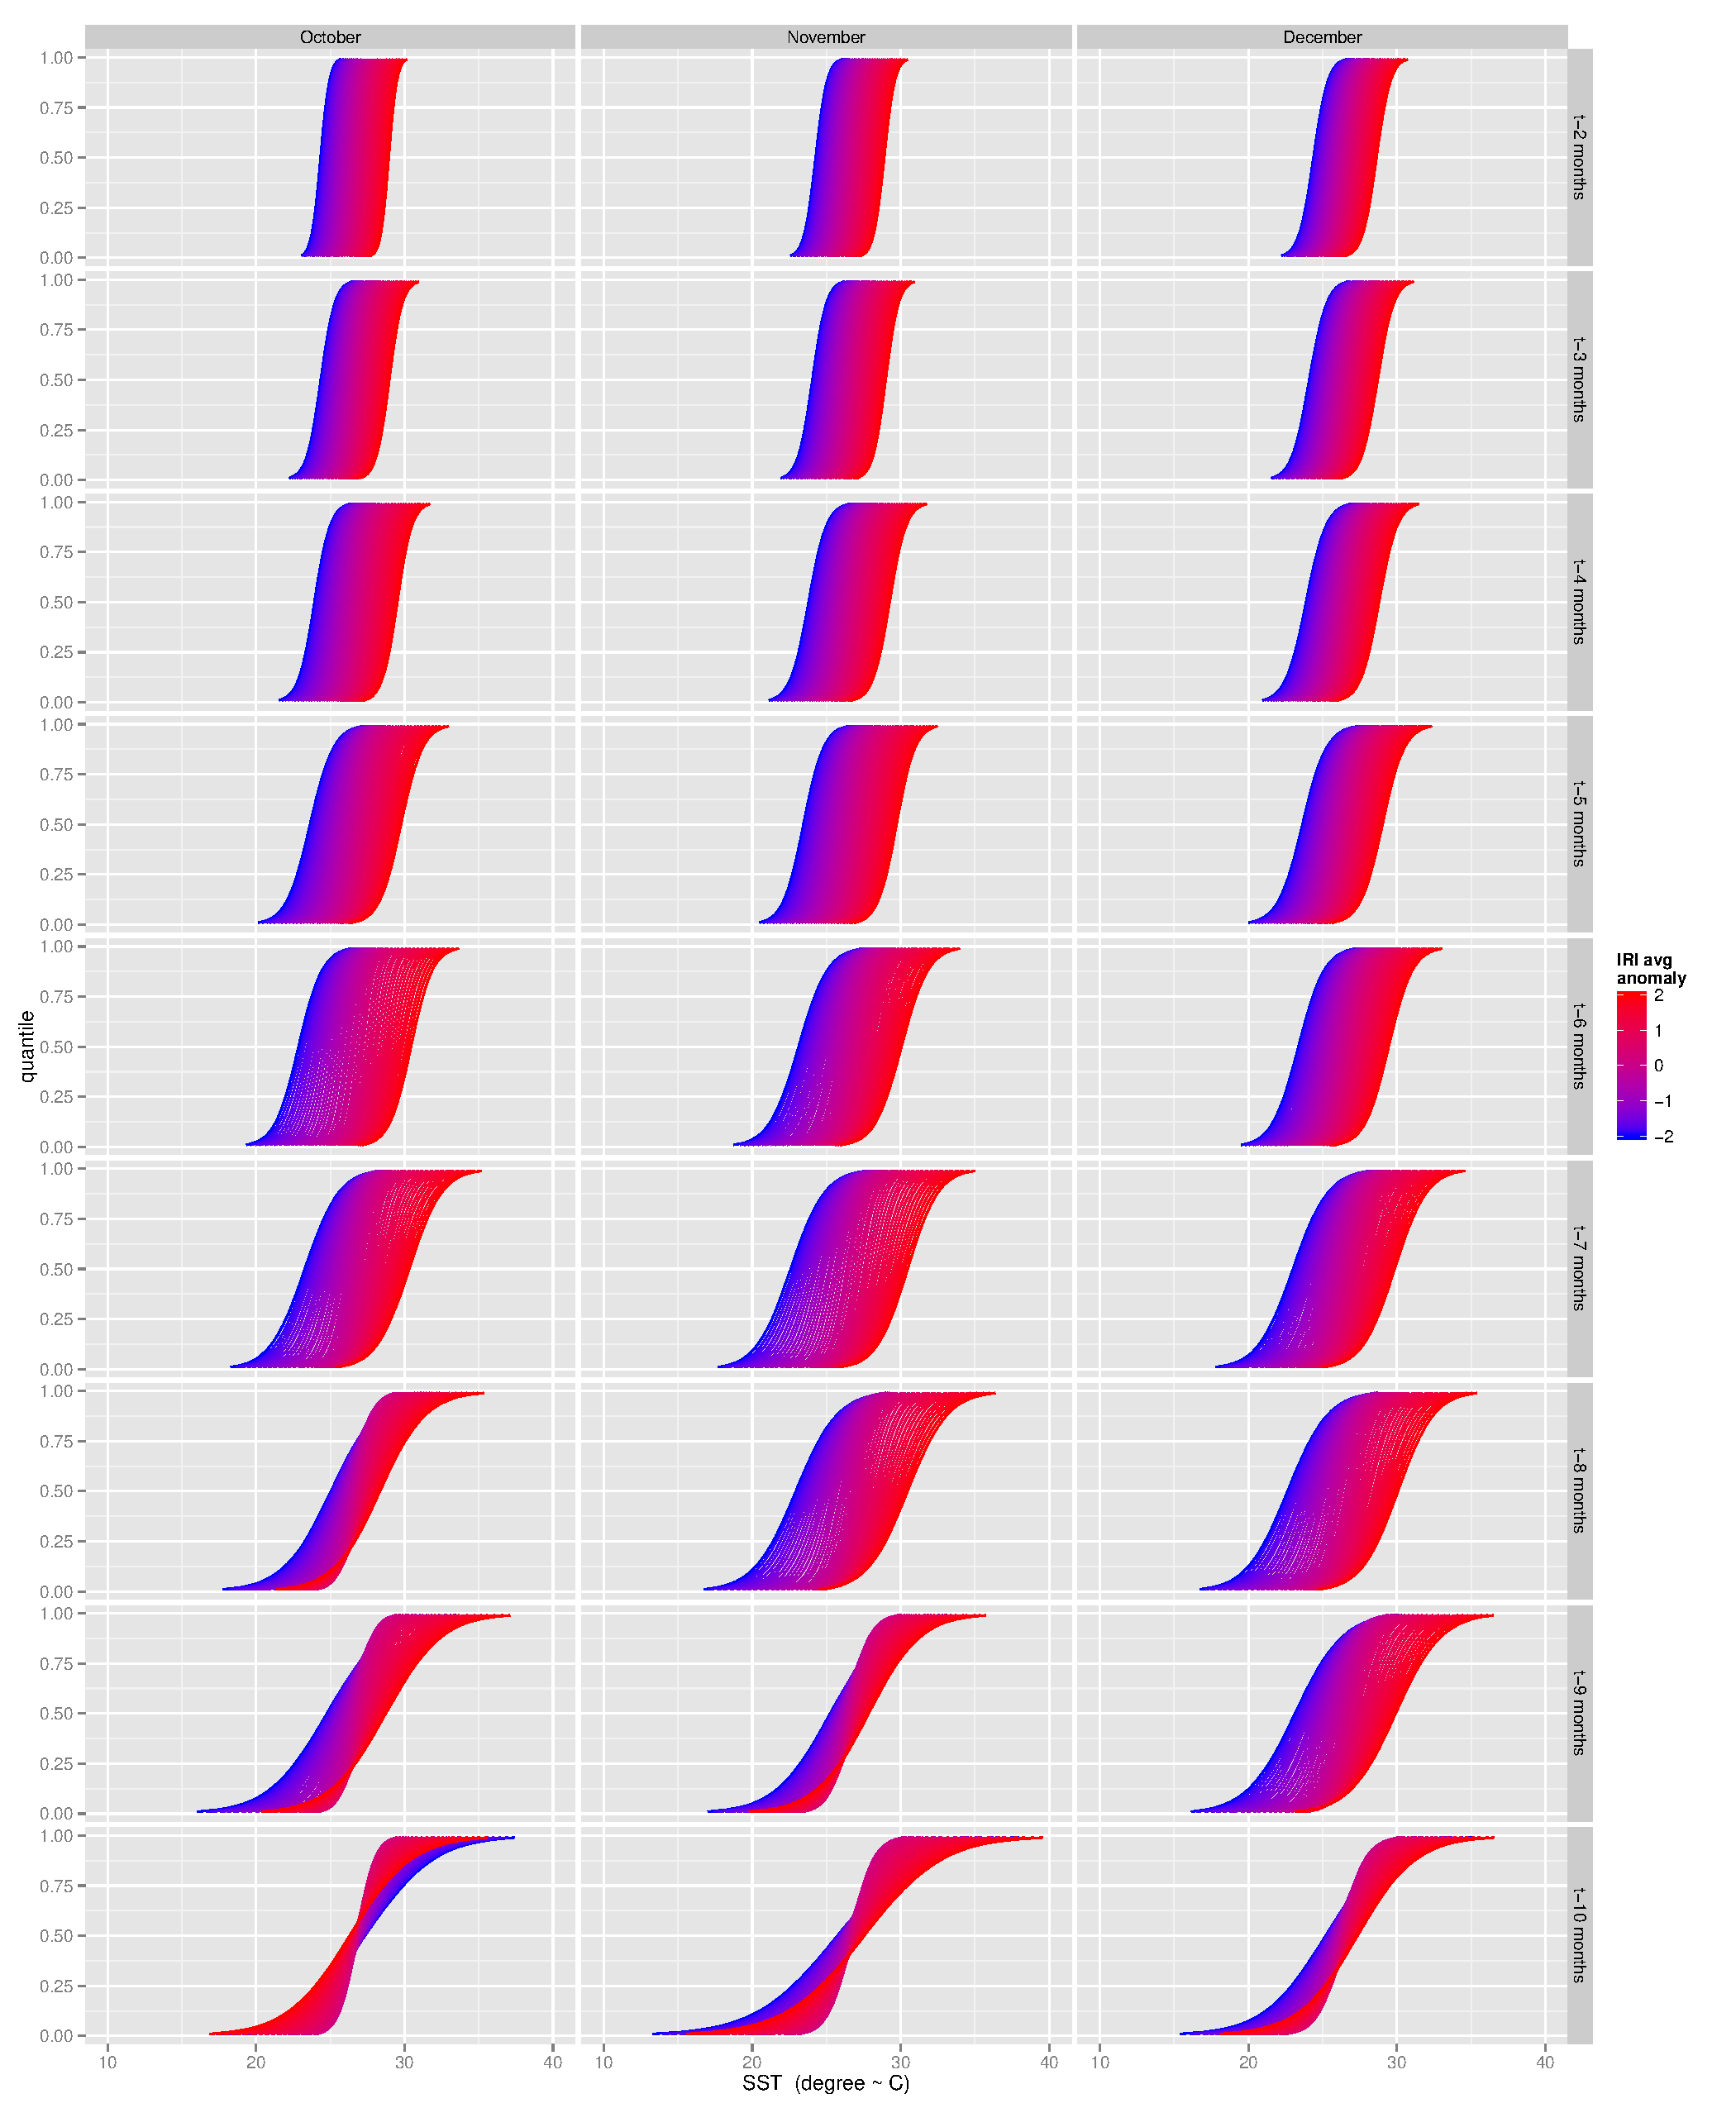
\includegraphics[width=\linewidth, keepaspectratio]{img/conditionalCDFs10to12TraditionalCDFconfig.pdf}
    \caption{Empirical cumulative distribution functions for October through December \text{Ni\~no} 3.4 SST conditioned on average IRI ensemble forecasts available for various months. ECDFs are of draws from the posterior predictive distribution of the model specified in equation \ref{eqn:conditionalEstEqn}.}
     \label{fig:conditionalCDFs10to12}
   \end{center}
\end{figure}

\begin{figure}[!htbp]
  \begin{center}
    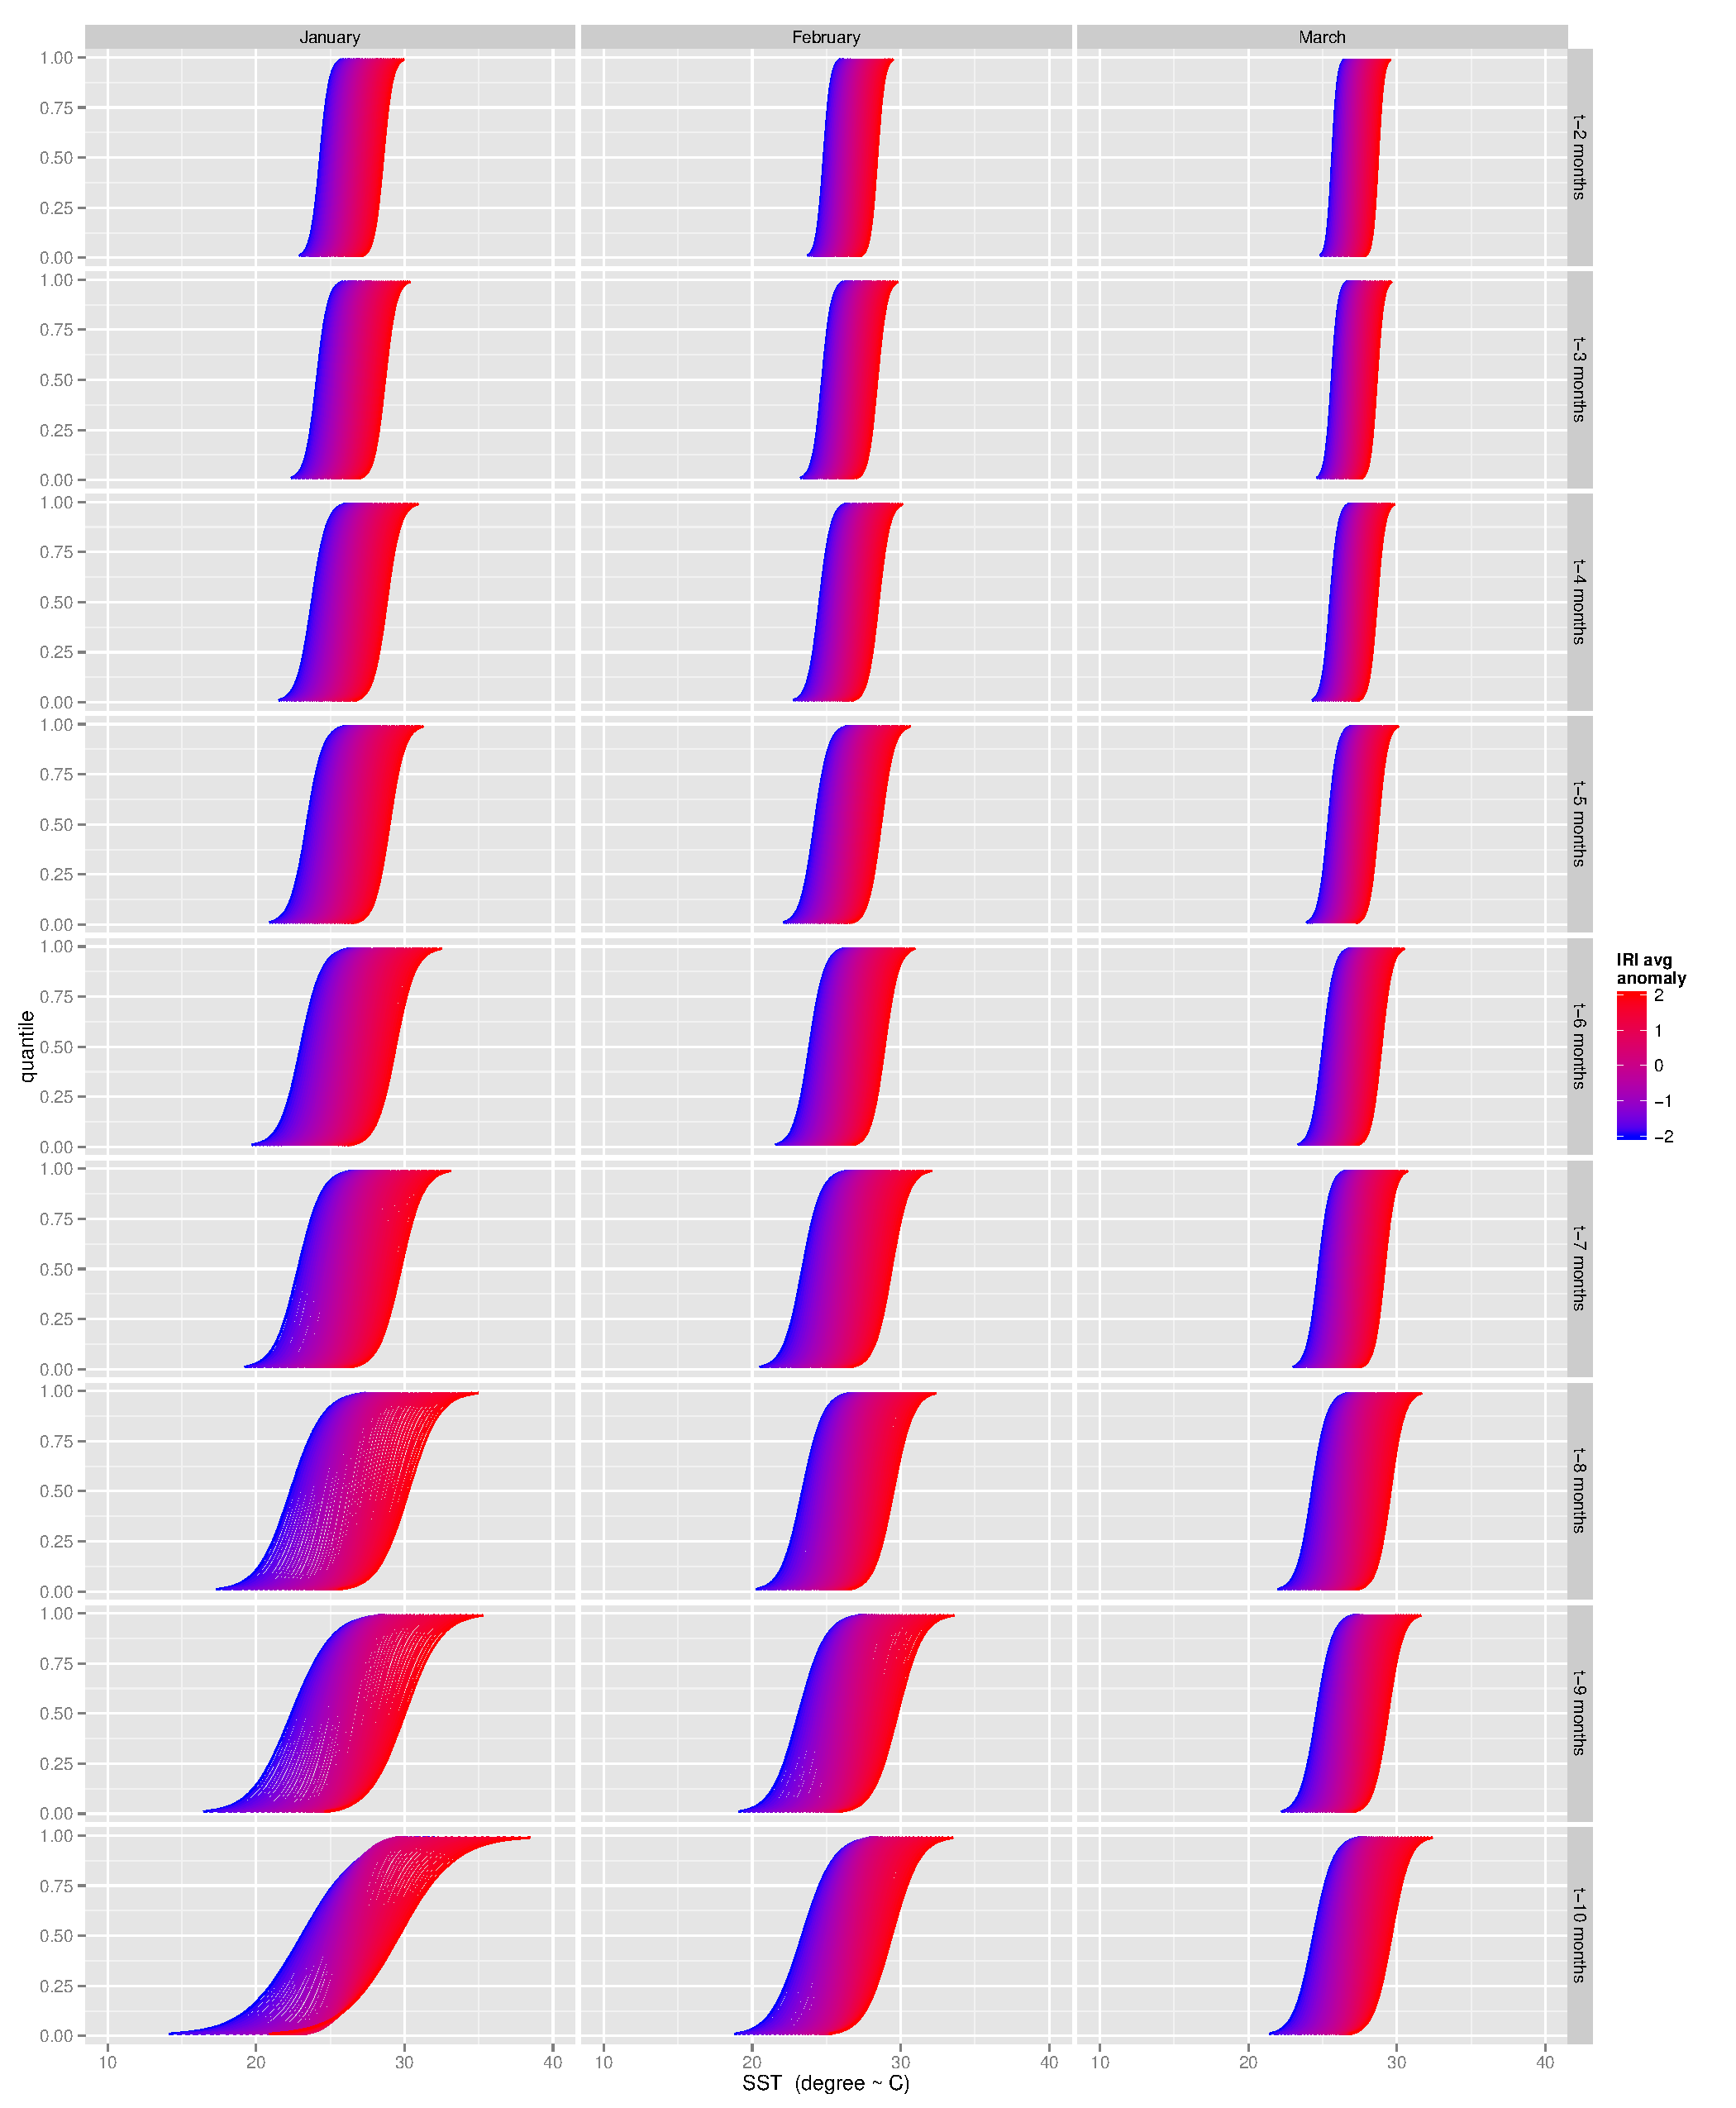
\includegraphics[width=\linewidth, keepaspectratio]{img/conditionalCDFs01to03TraditionalCDFconfig.pdf}
    \caption{Empirical cumulative distribution functions for January through March \text{Ni\~no} 3.4 SST conditioned on average IRI ensemble forecasts available for various months. ECDFs are of draws from the posterior predictive distribution of the model specified in equation \ref{eqn:conditionalEstEqn}.}
    \label{fig:conditionalCDFs01to03}
   \end{center}
\end{figure}

The spring predictive barrier is also clear in the figures. In the
October column of figure \ref{fig:conditionalCDFs10to12} red and blue
lines show substantial overlap for predictions made in February (8
months prior). By March, that pattern has vanished. Conditional on warm
and cold forecasts the probability distributions of eventual SST are
distinct, with the red and blue lines showing little overlap.

Notice that most of the ECDFs demonstrate their greatest spread along
the x-axis when they are furthest out from their target month. This
reflects the fact there there are relatively few long-dated extreme
forecasts in our sample. The diffuse priors on our parameters results in
high uncertainty for simulated outcomes when the sample size is small.
The model in equation \ref{eqn:conditionalEstEqn} allows for simulated
results that are much higher and lower than any observed SSTs in cases
where there are strong but unreliable forecasts.

\begin{table}[!htbp]
\centering \footnotesize
\begin{tabular}{rrrrrrrr}
  \hline
$\mbox{IRI anom}$ & $\mbox{price per USD}$ & $\mbox{E}[\mbox{SST}]$ & $2.5^{\mbox{th}}$ q & $25^{\mbox{th}}$ q & $50^{\mbox{th}}$ q & $75^{\mbox{th}}$ q & $97.5^{\mbox{th}}$ q \\ 
  \hline
-2.00 & 0.80 & 23.93 & 0.00 & 0.66 & 0.96 & 1.00 & 1.00 \\ 
  -1.90 & 0.77 & 24.07 & 0.00 & 0.59 & 0.89 & 1.00 & 1.00 \\ 
  -1.80 & 0.73 & 24.21 & 0.00 & 0.54 & 0.82 & 1.00 & 1.00 \\ 
  -1.70 & 0.68 & 24.35 & 0.00 & 0.47 & 0.75 & 1.00 & 1.00 \\ 
  -1.60 & 0.64 & 24.49 & 0.00 & 0.41 & 0.68 & 0.95 & 1.00 \\ 
  -1.50 & 0.58 & 24.63 & 0.00 & 0.34 & 0.60 & 0.87 & 1.00 \\ 
  -1.40 & 0.53 & 24.77 & 0.00 & 0.28 & 0.54 & 0.79 & 1.00 \\ 
  -1.30 & 0.47 & 24.91 & 0.00 & 0.21 & 0.47 & 0.71 & 1.00 \\ 
  -1.20 & 0.41 & 25.05 & 0.00 & 0.15 & 0.39 & 0.63 & 1.00 \\ 
  -1.10 & 0.35 & 25.19 & 0.00 & 0.08 & 0.32 & 0.55 & 1.00 \\ 
  -1.00 & 0.30 & 25.33 & 0.00 & 0.02 & 0.25 & 0.48 & 0.99 \\ 
  -0.90 & 0.24 & 25.47 & 0.00 & 0.00 & 0.18 & 0.40 & 0.90 \\ 
  -0.80 & 0.19 & 25.60 & 0.00 & 0.00 & 0.11 & 0.33 & 0.81 \\ 
  -0.70 & 0.15 & 25.74 & 0.00 & 0.00 & 0.03 & 0.25 & 0.72 \\ 
  -0.60 & 0.11 & 25.88 & 0.00 & 0.00 & 0.00 & 0.17 & 0.63 \\ 
  -0.50 & 0.08 & 26.02 & 0.00 & 0.00 & 0.00 & 0.10 & 0.55 \\ 
  -0.40 & 0.06 & 26.16 & 0.00 & 0.00 & 0.00 & 0.02 & 0.46 \\ 
  -0.30 & 0.04 & 26.30 & 0.00 & 0.00 & 0.00 & 0.00 & 0.38 \\ 
  -0.20 & 0.02 & 26.44 & 0.00 & 0.00 & 0.00 & 0.00 & 0.31 \\ 
  -0.10 & 0.02 & 26.58 & 0.00 & 0.00 & 0.00 & 0.00 & 0.23 \\ 
  0.00 & 0.01 & 26.72 & 0.00 & 0.00 & 0.00 & 0.00 & 0.16 \\ 
  0.10 & 0.01 & 26.86 & 0.00 & 0.00 & 0.00 & 0.00 & 0.08 \\ 
  0.20 & 0.00 & 26.99 & 0.00 & 0.00 & 0.00 & 0.00 & 0.01 \\ 
  0.30 & 0.00 & 27.14 & 0.00 & 0.00 & 0.00 & 0.00 & 0.00 \\ 
  0.40 & 0.00 & 27.27 & 0.00 & 0.00 & 0.00 & 0.00 & 0.00 \\ 
  0.50 & 0.00 & 27.41 & 0.00 & 0.00 & 0.00 & 0.00 & 0.00 \\ 
  0.60 & 0.00 & 27.55 & 0.00 & 0.00 & 0.00 & 0.00 & 0.00 \\ 
  0.70 & 0.00 & 27.69 & 0.00 & 0.00 & 0.00 & 0.00 & 0.00 \\ 
  0.80 & 0.00 & 27.83 & 0.00 & 0.00 & 0.00 & 0.00 & 0.00 \\ 
  0.90 & 0.00 & 27.97 & 0.00 & 0.00 & 0.00 & 0.00 & 0.00 \\ 
  1.00 & 0.00 & 28.11 & 0.00 & 0.00 & 0.00 & 0.00 & 0.00 \\ 
  1.10 & 0.00 & 28.24 & 0.00 & 0.00 & 0.00 & 0.00 & 0.00 \\ 
  1.20 & 0.00 & 28.38 & 0.00 & 0.00 & 0.00 & 0.00 & 0.00 \\ 
  1.30 & 0.00 & 28.53 & 0.00 & 0.00 & 0.00 & 0.00 & 0.00 \\ 
  1.40 & 0.00 & 28.67 & 0.00 & 0.00 & 0.00 & 0.00 & 0.00 \\ 
  1.50 & 0.00 & 28.80 & 0.00 & 0.00 & 0.00 & 0.00 & 0.00 \\ 
  1.60 & 0.00 & 28.95 & 0.00 & 0.00 & 0.00 & 0.00 & 0.00 \\ 
  1.70 & 0.00 & 29.08 & 0.00 & 0.00 & 0.00 & 0.00 & 0.00 \\ 
  1.80 & 0.00 & 29.23 & 0.00 & 0.00 & 0.00 & 0.00 & 0.00 \\ 
  1.90 & 0.00 & 29.36 & 0.00 & 0.00 & 0.00 & 0.00 & 0.00 \\ 
  2.00 & 0.00 & 29.51 & 0.00 & 0.00 & 0.00 & 0.00 & 0.00 \\ 
   \hline
\end{tabular}
\caption{Long put option spread (La Ni\~na protection) prices for October Ni\~no 3.4 SST conditioned on IRI ensemble forecasts released in June (strikes are set at one and three standard deviations below monthly average SSTs)} 
\label{tab:pricesOctSub}
\end{table}

Table \ref{tab:pricesOctSub}, translates simulation results into pricing
for October La \text{Ni\~na} protection (long put option spread
positions on October SST) conditioned on June forecasts using the payout
function discussed above (defined in equation \ref{eq:calloption} and
exemplified in figure \ref{fig:payouyt10callex}.) Notice that June is
well within the spring predictive barrier so forecasts of negative SST
anomalies greatly increase the expected value of La \text{Ni\~na}
protection. The full conditional pricing tables for all months, covering
both El \text{Ni\~no} and La \text{Ni\~na}, are avalible upon request
from the lead author\footnote{Pricing data will also soon be avaliable
  \href{www.directclimatemarkets.com}{here}.}.

\begin{figure}[!htbp]
\begin{center}
  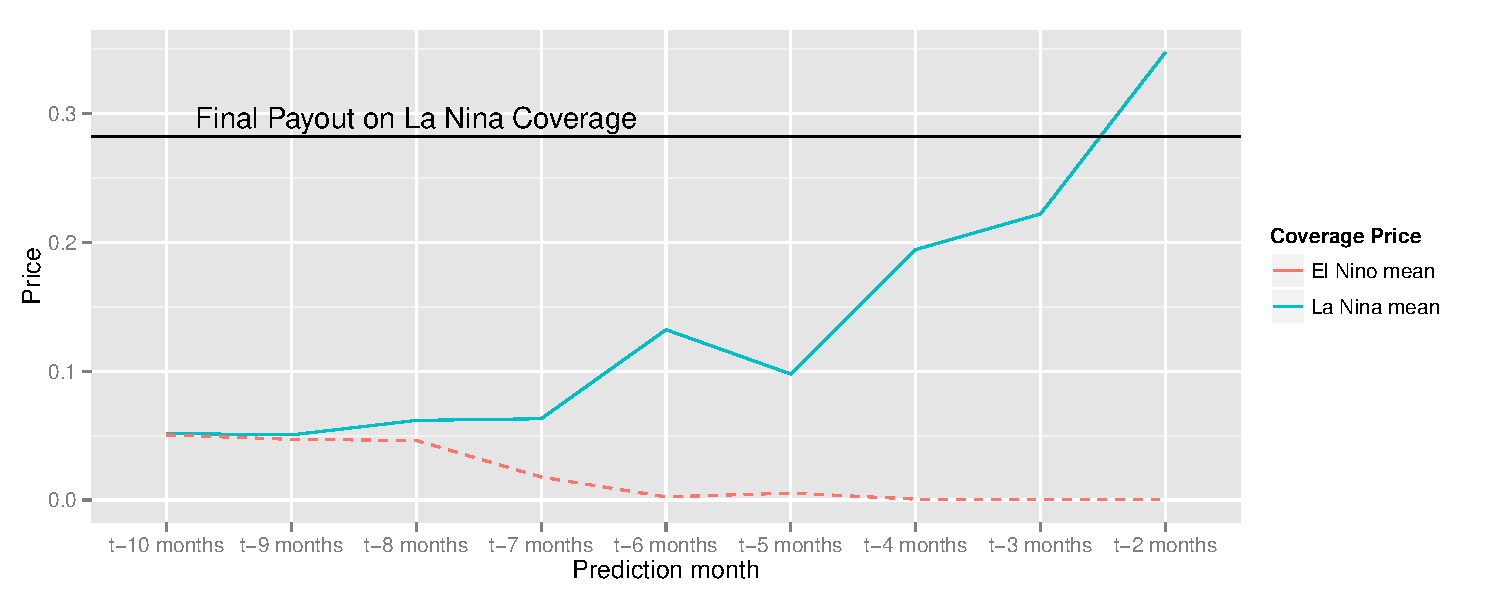
\includegraphics[width=\linewidth]{img/pricesOctober2010.pdf}
  \caption{Expected value of October 2010 La \text{Ni\~na} and El \text{Ni\~no} protection conditioned on available forecasts. Payout for actual October 2010 \text{Ni\~no} 3.4 SST in black.}
   \label{fig:pricesOctober2010}
      \end{center}
\end{figure}

\begin{figure}[!htbp]
\begin{center}
  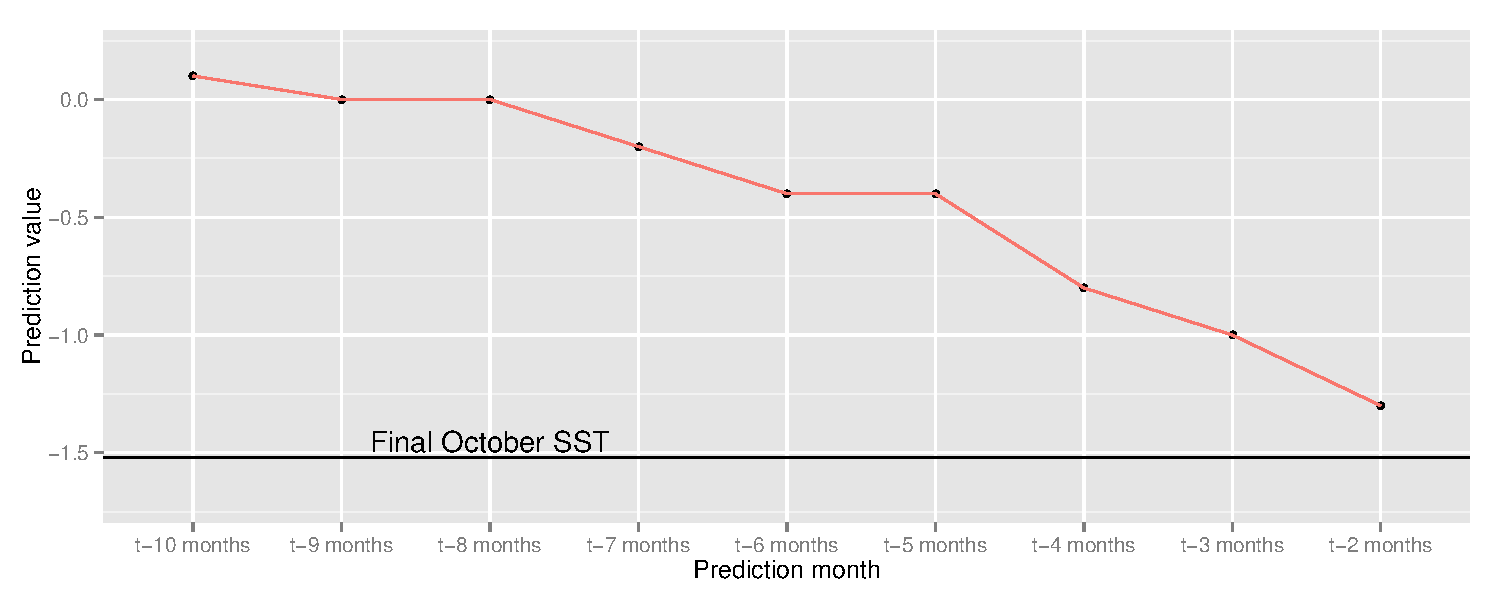
\includegraphics[width=\linewidth]{img/predOctober2010.pdf}
  \caption{IRI average anomaly forecast for October 2010. Actual October 2010 \text{Ni\~no} 3.4 SST anomaly in black.}
   \label{fig:predOctober2010}
   \end{center}
\end{figure}

We have also provided a price path for La \text{Ni\~na} and El
\text{Ni\~no} protection during the 2010 ENSO season, a season that
ultimately registered a negative anomaly of -1.52 degrees (a strong La
\text{Ni\~na}). Figure \ref{fig:pricesOctober2010} shows that expected
value of the two contracts is comparable until March (t-7 months) when
slightly negative forecasts from IRI (figure \ref{fig:predOctober2010}
erode the value of El \text{Ni\~no} protection. That parity of expected
values for standard El \text{Ni\~no} and La \text{Ni\~na} contracts is
of practical importance to hedgers who may wish to enter a costless
hedge position by, for example, selling El \text{Ni\~no} coverage and
using the proceeds to buy La \text{Ni\~na} coverage. (This is not
surprising given the terms of each contracts, which are structured
around one to three standard deviation anomalies in opposing
directions.) The opportunity to enter simple hedge positions at no
initial cost may be an additional incentive for businesses with
sophisticated and long-sighted risk management plans to enter their
hedges early in the season. Trades with no up-front capital required
will be available throughout the season, although not necessarily using
simple to interpret strikes.

La \text{Ni\~na} protection does not jump in value until April, by which
point El \text{Ni\~no} protection provides little expected value. After
May, when IRI forecasts hold steady and expected value falls, La
\text{Ni\~na} protection continues a steep climb in value throughout the
rest of the forecast season. While IRI forecasts head steadily downward,
the value of La \text{Ni\~na} protection appears to increase at an
increasing rate. In fact by August, forecasts suggest that the expected
payout will be above its ultimate settlement value. This suggests that
there would certainly be sufficient volatility to drive trading
throughout the forecast season in years with strong anomalies.

\begin{figure}[!htbp]
 \begin{center}
  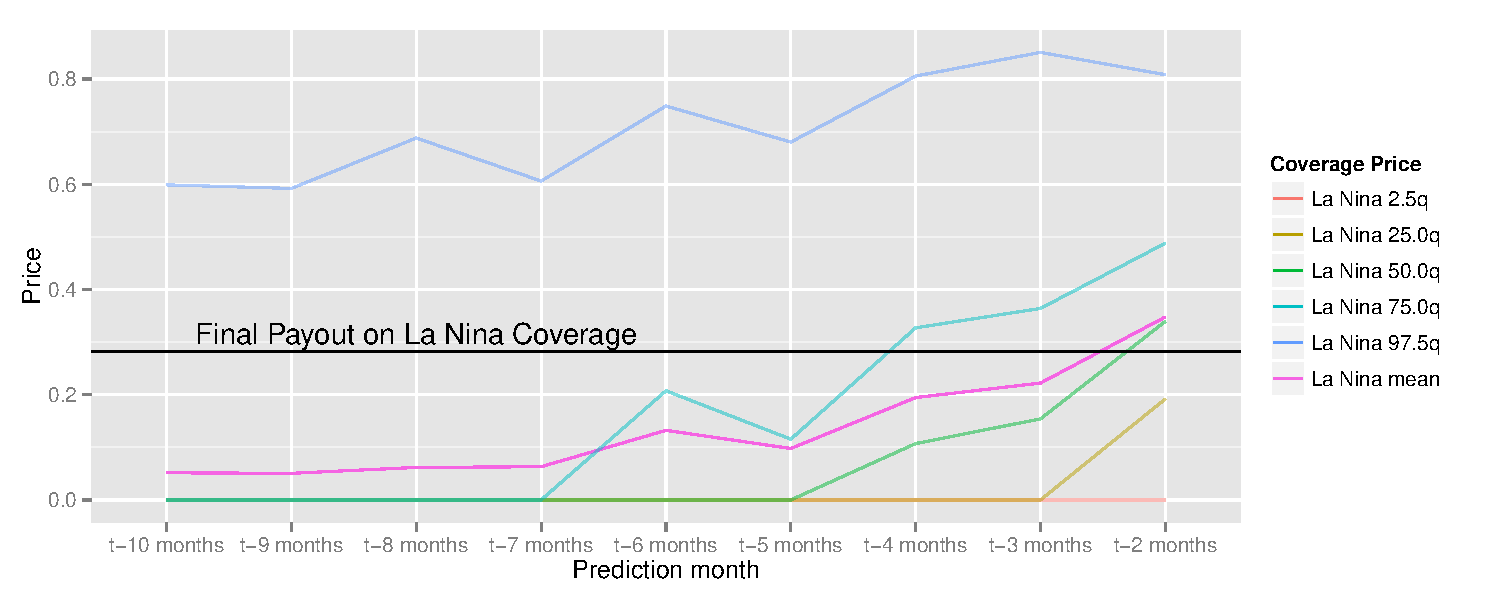
\includegraphics[width=\linewidth]{img/pricesOctober2010qs.pdf}
  \caption{Prices by quantile for October 2010 La \text{Ni\~na} protection conditioned on available forecasts. Payout for actual October 2010 \text{Ni\~no} 3.4 SST in black.}
   \label{fig:pricesOctober2010qs}
    \end{center}
\end{figure}

Figure \ref{fig:pricesOctober2010qs} provides simulation quantiles for
La \text{Ni\~na} contract values. This allows traders to see whether the
expected value of La \text{Ni\~na} coverage is driven by tail risks
(i.e.~only extreme show positive value) or the central tendencies of
simulated settlements (i.e.~the various quantiles are evenly spaced
across figure \ref{fig:pricesOctober2010qs}) in any given month. With
most of the simulations suggesting a settlement value of 0 until
April/May (only the 97.5th percentile of simulated results had positive
settlement value), the expected value of La \text{Ni\~na} protection in
early 2010 was driven by the risk of a surprise La \text{Ni\~na}. By
June, forecasts had fallen further while their informational value had
steadily risen, giving La \text{Ni\~na} protection a positive value in
most simulations. By August, most pricing benchmarks actually suggested
a value for La \text{Ni\~na} coverage that higher than the ultimate
payout.

Together figures \ref{fig:predOctober2010} and
\ref{fig:pricesOctober2010qs} show the flexibility of a stochastic
catalog of conditional prices for ENSO protection (shown in figures
\ref{fig:conditionalCDFs04to06}, \ref{fig:conditionalCDFs07to09},
\ref{fig:conditionalCDFs10to12}, and \ref{fig:conditionalCDFs01to03})).
They also demonstrate how information is more important at some points
in the forecast cycle than others. In 2010, El \text{Ni\~no} and La
\text{Ni\~na} protection are roughly equivalent in value until we passed
the spring predictive barrier. 2010's first actionable forecasts showed
only slightly colder-than-normal SSTs (figure
\ref{fig:predOctober2010}). However, that was sufficient to preserve the
option value of La \text{Ni\~na} protection (figure
\ref{fig:pricesOctober2010qs}) and rapidly erode the value of El
\text{Ni\~no} protection. Figures \ref{fig:predOctober2010} and
\ref{fig:predOctober2010qs} demonstrate how better early forecasting
information could lead to economic efficiency gains as the price of ENSO
spread positions will rise or fall in value earlier in the forecasting
season. Currently, early forecasts for October (prior to the spring
predictive barrier) are insufficient to move the expected value of risk
protection.

The prices in show in this article and available upon request from the
lead author only reflect the underlying risk of the index. In actual
transactions, these pure risk prices will generally be:

\begin{itemize}
\itemsep1pt\parskip0pt\parsep0pt
\item
  adjusted (downward) to reflect the time value of the premium paid by
  hedgers;
\item
  subjected to some margining\footnote{Margining refers to the process
    of setting aside collateral on financial trades. On exchange-traded
    derivatives there are clear, predictable rules for how much money
    must be set aside as collateral in a \emph{margin account} as the
    trade's settlement index changes over time.} rules, when applicable;
  and
\item
  adjusted (upward) to allow for some reasonable expected profit for
  speculators.
\end{itemize}

Those adjustments are routine in financial markets and not addressed in
this article.

\section{Conclusion}\label{conclusion}

Climate risks are difficult to hedge in existing markets. To address
that market gap, this article proposed markets based on indexes of
regional climate anomalies with long-range physical and statistical
links to extreme weather events, known to climate scientists as
teleconnections.

Looking at El \text{Ni\~no}-Southern Oscillation (ENSO), the one
regional climate anomaly already manged through insurance in Peru, we
discuss the nature of teleconnection risk and how that might inform its
transition to markets. Of particular interest is how the asymmetric
information that undermines existing insurance markers in ENSO risk, may
be welfare enhancing when channeled into price discovery.

Having identified the value of traded markets covering teleconnection
risk, we provide a framework and tools to incubate that risk trading. We
walk through practical considerations for the statistical modeling
showing, for example, how distributional assumptions about ENSO may have
serious implications for the price of risk protection. We also place
prices on ENSO forecast uncertainty while developing stochastic catalogs
of ENSO anomalies. Using those catalogs we showed likely patterns in
ENSO risk trading, demonstrating, among other things, that there is
actionable information emerging throughout the likely ENSO trading
season. That information is sufficient to drive the active trading
needed for reliable price discovery.

For direct climate markets, like ENSO, to come to fruition academic
research must be supported by institutional innovations. For example,
National Meteorological Services like NOAA should have a simple system
for licensing the indexes they produce for use in financial contracts.
Licensing revenues are unlikely to be large enough to support
substantially expanded research teams to maintain, upgrade, and expand
index offerings. However, they could provide valuable support to the
specific research teams that are generating great social value.

By funding the research teams that produce indexes of climate, national
governments already provide implicit support to potential markets like
ENSO. However, given the public good nature of the forecasts these
markets could generate and their fundamental link to government
research, it may be economically efficient to explicitly subsidize the
emergence of direct climate markets through challenge grants.

\section*{References}\label{references}
\addcontentsline{toc}{section}{References}

Agbroko, R. 2012. \emph{Cocoa at Nine-Month High in Weather Fear},
\{August 1\}.

Aranda, M. 2009. ``Evolution and State of the Art of Fishing Capacity
Management in Peru: The Case of the Anchoveta Fishery.''
\emph{Pan-American Journal of Aquatic Sciences} 4 (2): 146--53.

Ashok, K., S.K. Behera, S.A. Rao, H. Weng, and T. Yamagata. 2007. ``El
Ni\textasciitilde{}no Modoki and Its Possible Teleconnection.''
\emph{Journal of Geophysical Research: Oceans} 112 (C11).

Barnston, A.G., M. Chelliah, and S.B. Goldenberg. 1997. ``Documentation
of a Highly ENSO-Related SST Region in the Equatorial Pacific.''
\emph{Atmosphere Ocean} 35 (3). Ottawa, Ont.: Canadian Meteorological;
Oceanographic Society: 367.

Black, D.G. 1986. ``Success and Failure of Futures Contracts: Theory and
Empirical Evidence.'' PhD thesis, New York University. Graduate School
of Business Administration. Salomon Brothers Center for the Study of
Financial Institutions.

Brorsen, B.W., and N.F. Fofana. 2001. ``Success and Failure of
Agricultural Futures Contracts.'' \emph{Journal of Agribusiness} 19 (2).
The Agricultural Economics Association of Georgia: 129--46.

Carlton, D.W. 1984. ``Futures Markets: Their Purpose, Their History,
Their Growth, Their Successes and Failures.'' \emph{Journal of Futures
Markets} 4 (3). Wiley Online Library: 237--71.

Cavanaugh, G., B. Collier, and J.R. Skees. 2010. ``Incorporating Weather
Index Insurance with Territorial Approaches to Climate Change (TACC) in
Northern Peru.'' United Nations Development Programme; GlobalAgRisk.

Cavanaugh, Grant. 2013. ``Chapter 7: Interviews with Risk
Professionals.'' \url{directclimatemarkets.com}.

Chiew, F.H.S., T.C. Piechota, J.A. Dracup, and T.A. McMahon. 1998. ``El
Ni\textasciitilde{}no/Southern Oscillation and Australian Rainfall,
Streamflow and Drought: Links and Potential for Forecasting.''
\emph{Journal of Hydrology} 204 (1). Elsevier: 138--49.

Chincarini, L. 2011. ``No Chills or Burns from Temperature Surprises: An
Empirical Analysis of the Weather Derivatives Market.'' \emph{Journal of
Futures Markets} 31 (1): 1--33.

Clarke, A.J. 2008. \emph{An Introduction to the Dynamics of El Nino \&
the Southern Oscillation}. Academic Press.

CME Group. 2014. ``CME Hurricane Index Futures and Options.''
\url{\{cmegroup.com/trading/weather/files/WT106NEWHurricaneFC.pdf\}}.

Coelho, CAS, S Pezzulli, M Balmaseda, F.J. Doblas-Reyes, and D.B.
Stephenson. 2004. ``Forecast Calibration and Combination: A Simple
Bayesian Approach for ENSO.'' \emph{Journal of Climate} 17 (7):
1504--16.

Collier, B.L., and J.R. Skees. 2013. ``Exclusive Finance: How Unmanaged
Systemic Risk Continues to Limit Financial Services for the Poor in a
Booming Sector.'' Wharton Risk Management; Decision Processes Center.

Copeland, T.E., and D. Galai. 1983. ``Information Effects on the Bid-Ask
Spread.'' \emph{Journal of Finance} 38 (5): 1457--69.

Cummins, J.D., and S. Tennyson. 1992. ``Controlling Automobile Insurance
Costs.'' \emph{The Journal of Economic Perspectives}. JSTOR, 95--115.

Duffie, D., and M.O. Jackson. 1989. ``Optimal Innovation of Futures
Contracts.'' \emph{Review of Financial Studies} 2 (3): 275--96.

Ederington, L.H. 1979. ``The Hedging Performance of the New Futures
Markets.'' \emph{The Journal of Finance} 34 (1): 157--70.

Electric Reliability Council of Texas (ERCOT). 2014. ``Seasonal
Updates.'' \url{http://www.ercot.com/about/weather/updates.html}.

Evans, S. 2013. ``Beyond Price, Pressure Increasingly Seen on
Reinsurance Terms: PartnerRe CEO.''
\url{http://www.artemis.bm/blog/2014/11/03/beyond-price-pressure-increasingly-seen-on-reinsurance-terms-partnerre-ceo/}.

Fowler, HJ, S Blenkinsop, and C Tebaldi. 2007. ``Linking Climate Change
Modelling to Impacts Studies: Recent Advances in Downscaling Techniques
for Hydrological Modelling.'' \emph{International Journal of
Climatology} 27 (12). Wiley Online Library: 1547--78.

Froot, K. 1999. \emph{The Financing of Catastrophe Risk}. University of
Chicago Press.

Froot, K.A. 2001. ``The Market for Catastrophe Risk: A Clinical
Examination.'' \emph{Journal of Financial Economics} 60 (2): 529--71.

Gladwin, H., and W.G. Peacock. 1997. \emph{Warning and Evacuation: A
Night for Hard Houses}. \emph{Hurricane Andrew: Gender, Ethnicity and
the Sociology of Disasters}. Routledge, New York.

Glantz, M.H., R.W. Katz, and N. Nicholls. 1991. \emph{Teleconnections
Linking Worldwide Climate Anomalies.} Cambridge, UK.

Glosten, L.R., and P.R. Milgrom. 1985. ``Bid, Ask and Transaction Prices
in a Specialist Market with Heterogeneously Informed Traders.''
\emph{Journal of Financial Economics} 14 (1): 71--100.

Gorham, M., and P. Kundu. 2012. ``A Half-Century of Product Innovation
and Competition at U.S. Futures Exchanges.'' \emph{The Review of Futures
Markets} 20 (July): 105--40.

Gray, Roger W. 1978. ``Why Does Futures Trading Succeed or Fail: An
Analysis of Selected Commodities.'' \emph{Readings in Futures Markets:
Views from the Trade}. Chicago Board of Trade.

Haug, E.G., and N.N. Taleb. 2011. ``Option Traders Use (Very)
Sophisticated Heuristics, Never the Black--Scholes--Merton Formula.''
\emph{Journal of Economic Behavior \& Organization} 77 (2). Elsevier:
97--106.

{IPCC}, {Intergovernmental Panel on Climate Change - Working Group I}.
2013. \emph{Fifth Assessment Report, Climate Change 2013: The Physical
Science Basis}. Intergovernmental Panel on Climate Change.

Jacquet, Jennifer., K. Hagel, C. Hauert, J. Marotzke, T. R{ö}hl, and M.
Milinski. 2013. ``Intra-and Intergenerational Discounting in the Climate
Game.'' \emph{Nature Climate Change}. Nature Publishing Group.

Jewson, S., and A. Brix. 2005. \emph{Weather Derivative Valuation: The
Meteorological, Statistical, Financial and Mathematical Foundations}.
Cambridge University Press.

Khalil, A.F., H. Kwon, U. Lall, M.J. Miranda, and J.R. Skees. 2007. ``El
Ni\textasciitilde{}no-Southern Oscillation-Based Index Insurance for
Floods: Statistical Risk Analyses and Application to Peru.'' \emph{Water
Resources Research} 43 (10). American Geophysical Union: 10416.

Klotzbach, P.J. 2011. ``El Ni\textasciitilde{}no-Southern Oscillation's
Impact on Atlantic Basin Hurricanes and US Landfalls.'' \emph{Journal of
Climate} 24 (4): 1252--63.

Kurtov, A., ed. 2010. \emph{Investing in Insurance Risk:
Insurance-Linked Securities - a Practitioner's Perspective}. Risk Books.

Kyle, A.S. 1985. ``Continuous Auctions and Insider Trading.''
\emph{Econometrica: Journal of the Econometric Society}, 1315--35.

Lagos, P., Y. Silva, E. Nickl, and K. Mosquera. 2008. ``El
Ni\textasciitilde{}no-Related Precipitation Variability in Perú.''
\emph{Advances in Geosciences} 14: 231--37.

Leland, H.E. 1992. ``Insider Trading: Should It Be Prohibited?''
\emph{Journal of Political Economy}, 859--87.

Luo, L., E.F. Wood, and M. Pan. 2007. ``Bayesian Merging of Multiple
Climate Model Forecasts for Seasonal Hydrological Predictions.''
\emph{Journal of Geophysical Research: Atmospheres} 112 (D10).

Nordhaus, W. 2013. \emph{The Climate Casino}. Yale University Press.

Pennings, J.M.E., and R.M. Leuthold. 1999. \emph{Commodity Futures
Contract Viability: A Multidisciplinary Approach}. Vol. 51. University
of Illinois, Champagne-Urbana.

---------. 2000. ``The Motivation for Hedging Revisited.'' \emph{Journal
of Futures Markets} 20 (9). Wiley Online Library: 865--85.

---------. 2001. ``A Behavioural Approach Towards Futures Contract
Usage.'' \emph{Australian Economic Papers} 40 (4). Wiley Online Library:
461--78.

Pindyck, R.S. 2013. \emph{Climate Change Policy: What Do the Models Tell
Us?} National Bureau of Economic Research.

Reynolds, R.W., and D.C. Marsico. 1993. ``An Improved Real-Time Global
Sea Surface Temperature Analysis.'' \emph{Journal of Climate} 6 (1):
114--19.

Reynolds, R.W., and T.M. Smith. 1994. ``Improved Global Sea Surface
Temperature Analyses Using Optimum Interpolation.'' \emph{Journal of
Climate} 7 (6): 929--48.

Reynolds, R.W., N.A. Rayner, T.M. Smith, D.C. Stokes, and W. Wang. 2002.
``An Improved in Situ and Satellite SST Analysis for Climate.''
\emph{Journal of Climate} 15 (13): 1609--25.

Reynolds, Richard W. 1988. ``A Real-Time Global Sea Surface Temperature
Analysis.'' \emph{Journal of Climate} 1 (1): 75--86.

Roll, R. 1984. ``Orange Juice and Weather.'' \emph{American Economic
Review} 74 (5). American Economic Association: 861--80.

Ropelewski, C.F., and M.S. Halpert. 1987. ``Global and Regional Scale
Precipitation Patterns Associated with the El
Ni\textasciitilde{}no/Southern Oscillation.'' \emph{Monthly Weather
Review} 115 (8): 1606--26.

---------. 1989. ``Precipitation Patterns Associated with the High Index
Phase of the Southern Oscillation.'' \emph{Journal of Climate} 2:
268--84.

Rosenzweig, C., and D. Hillel. 2008. \emph{Climate Variability and the
Global Harvest: Impacts of El Ni\textasciitilde{}no and Other
Oscillations on Agro-Ecosystems}. Oxford University Press, USA.

Sandor, R. 2012. \emph{Good Derivatives: A Story of Financial and
Environmental Innovation}. John Wiley; Sons.

Scholes, Myron S. 1998. ``Derivatives in a Dynamic Environment.''
\emph{American Economic Review}, 350--70.

Schultz, P. 2012. \emph{Insurance-Linked Securities}. Aon Benfield
Securities. \url{http://thoughtleadership.aonbenfield.com/}.

Silber, W.L. 1981. ``Innovation, Competition, and New Contract Design in
Futures Markets.'' \emph{Journal of Futures Markets} 1 (2). Wiley Online
Library: 123--55.

Skees, J.R. 2013. ``First Ever 'Forecast Insurance' Offered for Extreme
El in Peru.''
\url{http://globalagrisk.com/Pubs/2013\%20Press\%20Release_First_Ever\%20_Forecast\%20Insurance\%20Peru.pdf}.

Skees, J.R., and A.G. Murphy. 2009. ``ENSO Business Interruption Index
Insurance for Catastrophic Flooding in Piura, Peru.''

Skees, J.R., J.R. Black, and B.J. Barnett. 1997. ``Designing and Rating
an Area Yield Crop Insurance Contract.'' \emph{American Journal of
Agricultural Economics} 79 (2). Oxford University Press: 430--38.

Skees, J.R., J. Hartell, and A.G. Murphy. 2007. ``Using Index-Based Risk
Transfer Products to Facilitate Micro Lending in Peru and Vietnam.''
\emph{American Journal of Agricultural Economics} 89 (5): 1255--61.

Smith, T.M., and R.W. Reynolds. 2003. ``Extended Reconstruction of
Global Sea Surface Temperatures Based on COADS Data (1854-1997).''
\emph{Journal of Climate} 16 (10): 1495--1510.

---------. 2004. ``Improved Extended Reconstruction of SST
(1854-1997).'' \emph{Journal of Climate} 17 (12): 2466--77.

Smith, T.M., R.W. Reynolds, T.C. Peterson, and J. Lawrimore. 2008.
``Improvements to NOAA's Historical Merged Land-Ocean Surface
Temperature Analysis (1880-2006).'' \emph{Journal of Climate} 21 (10):
2283--96.

Stan Development Team. 2013. ``Stan: A C++ Library for Probability and
Sampling, Version 1.3.'' \url{http://mc-stan.org/}.

Swiss Re. 2012. \emph{Insurance-Linked Securities Market Update}. Swiss
Re Capital Markets Insurance-Linked Securities.
\url{http://media.swissre.com/documents/SRCM_ILS_Market_Update_Jan2012.pdf}.

Tashjian, E. 1995. ``Optimal Futures Contract Design.'' \emph{The
Quarterly Review of Economics and Finance} 35 (2). Elsevier: 153--62.

The Economist. 2013. ``Carbon Trading: ETS, RIP?'' \emph{The Economist},
\{April 20\}.

Ursano, Tony. 2013. \emph{ILS Market Update}. Willis Captial Markets \&
Advisory.
\url{http://www.willis.com/Documents/Publications/Services/WCMA/WCMA_May_2013_ILS_Market_Update.pdf}.

Woo, Gordon. 1999. \emph{The Mathematics of Natural Catastrophes}. World
Scientific.

Working, H. 1953. ``Futures Trading and Hedging.'' \emph{The American
Economic Review} 43 (3). JSTOR: 314--43.

Xue, Y., T.M. Smith, and R.W. Reynolds. 2003. ``Interdecadal Changes of
30-Yr SST Normals During 1871-2000.'' \emph{Journal of Climate} 16 (10):
1601--12.

\end{document}

